\chapter{Architecture de la solution}

\section{Introduction}

L’analyse automatisée de matchs sportifs à partir de flux vidéo constitue une problématique pluridisciplinaire située à l’intersection de la vision par ordinateur, de l’apprentissage automatique et de la modélisation géométrique. Dans le cas spécifique du padel, cette problématique présente une complexité accrue en raison de plusieurs facteurs : la vitesse élevée de la balle, la densité des échanges, les interactions simultanées entre quatre joueurs, ainsi que les multiples réflexions de la balle sur les parois vitrées du terrain. L’enjeu consiste donc à transformer un simple flux vidéo en un ensemble de données structurées, fiables et exploitables, tout en respectant les contraintes de précision et de traitement en temps réel.

Afin de répondre à ces exigences, nous avons conçu SmartPlayAI, une plateforme intelligente d’analyse vidéo dédiée au padel. L’architecture du système repose sur un pipeline modulaire dans lequel chaque composant remplit une fonction clairement définie et produit des résultats exploités par les modules situés en aval. Les choix technologiques effectués ont été guidés par une étude comparative des solutions existantes, dans le but d’obtenir le meilleur compromis entre précision, robustesse et efficacité computationnelle.

Ce chapitre présente l’architecture globale de SmartPlayAI ainsi que les principaux choix de conception ayant guidé son développement. Nous décrirons les différents modules qui composent le système et leur rôle dans le processus d’analyse, depuis le traitement des vidéos jusqu’à la génération des statistiques et des visualisations.
\section{Architecture générale du système}

Avant de détailler le fonctionnement de chaque module, il est nécessaire de présenter le système dans son ensemble. Pour cela, nous adoptons une approche classique en ingénierie logicielle reposant sur deux niveaux de description complémentaires : une vue externe, dite \textit{boîte noire}, qui met en évidence les entrées et les sorties du système, et une vue interne, dite \textit{boîte blanche}, qui expose l’organisation des composants ainsi que leurs interactions.

\subsection{Vue externe du système (boîte noire)}

Du point de vue de l’utilisateur final, SmartPlayAI se comporte comme un système à entrée unique et à sorties multiples. En entrée, il reçoit un flux vidéo d’un match de padel, capturé à une fréquence comprise entre 25 et 30 images par seconde. En sortie, il génère un ensemble de données analytiques structurées et visualisations enrichies.

\begin{figure}[H]
    \centering
    \resizebox{\textwidth}{!}{%
    \begin{tikzpicture}[
        node distance=2cm,
        every node/.style={font=\small},
        input/.style={draw, rounded corners, fill=blue!10, minimum width=3.5cm, minimum height=1.5cm, align=center},
        system/.style={draw, rounded corners, fill=green!10, minimum width=4cm, minimum height=2cm, align=center, font=\bfseries},
        output/.style={draw, rounded corners, fill=orange!10, minimum width=4.5cm, minimum height=5cm, align=left}
    ]
    \node[input] (video) {Flux vidéo\\Match de padel};
    \node[system, right=of video] (system) {SmartPlayAI};
    \node[output, right=of system] (output) {
        \textbf{Sorties générées :}\\[0.2cm]
        • Trajectoires joueurs\\
        • Trajectoire balle\\
        • Statistiques avancées\\
        • Heatmaps\\
        • Événements de jeu\\
        • CSV\\
        • JSON\\
        • MP4 annoté
    };
    \draw[-{Latex[length=4mm]}, thick] (video) -- (system);
    \draw[-{Latex[length=4mm]}, thick] (system) -- (output);
    
    \end{tikzpicture}%
    }
    \caption{Vue externe (boîte noire) de SmartPlayAI}
    \label{fig:blackbox-smartplayai}
\end{figure}

Les résultats produits par le système peuvent être regroupés selon trois axes complémentaires : la richesse des informations extraites, la diversité des formats de sortie et la flexibilité du mode de traitement.

\subsection{Vue interne du système (boîte blanche)}

Sur le plan interne, SmartPlayAI est organisé sous la forme d’un pipeline de traitement parallèle composé de neuf blocs fonctionnels. Chaque bloc est spécialisé dans une tâche précise et transmet ses résultats aux modules suivants.

\begin{figure}[H]
    \centering
    \maybeincludegraphics[width=0.9\textwidth]{images_chap2/boite_blanche.png}
    \caption{Vue interne (boîte blanche) de SmartPlayAI}
    \label{fig:whitebox-smartplayai}
\end{figure}

\subsection{Composants principaux}

\begin{table}[H]
\centering
\caption{Composants principaux de SmartPlayAI et technologies associées}
\label{tab:components-smartplayai}
\renewcommand{\arraystretch}{1.3}
\begin{tabular}{|p{3.5cm}|p{6cm}|p{3.5cm}|}
\hline
\textbf{Composant} & \textbf{Rôle fonctionnel} & \textbf{Technologie retenue} \\
\hline
Détection des joueurs & Localiser et délimiter chaque joueur & YOLO26 \\
\hline
Analyse de posture & Extraire les 17 points clés du squelette & YOLOv8-Pose \\
\hline
Détection de la balle & Estimer la trajectoire spatio-temporelle & TrackNetV3 \\
\hline
Modélisation du terrain & Détecter les lignes et coins du court & YOLOv8 Keypoints \\
\hline
Segmentation des joueurs & Isoler précisément les silhouettes & SAM2 \\
\hline
Suivi multi-objets & Maintenir des identifiants stables & ByteTrack \\
\hline
Projection homographique & Convertir les coordonnées image en coordonnées métriques & OpenCV \\
\hline
Analyse événementielle & Détecter les services, frappes et fautes & Automate à états finis \\
\hline
Visualisation et Dashboard & Afficher statistiques et heatmaps & Streamlit + Pandas \\
\hline
\end{tabular}
\end{table}

\subsection{Flux de données et intégration des modules}

Le flux de données dans SmartPlayAI suit une logique séquentielle à l’échelle du pipeline complet, mais parallèle à l’échelle de chaque image. Les données issues des modules de détection sont normalisées puis converties dans le référentiel physique du terrain par projection homographique.

\begin{figure}[H]
    \centering
    \resizebox{\textwidth}{!}{%
    \begin{tikzpicture}[
        every node/.style={font=\small},
        block/.style={draw, rounded corners, fill=blue!10, minimum width=3.2cm, minimum height=1.3cm, align=center}
    ]
    \node[block] (frame) at (0,0) {Image\\(Frame t)};
    \node[block] (detect) at (4,0) {Détection\\parallèle};
    \node[block] (aggregate) at (8,0) {Agrégation\\des résultats};
    \node[block] (homo) at (12,0) {Projection\\homographique};
    \node[block] (analysis) at (16,0) {Scoring et\\statistiques};

    \draw[-{Latex[length=4mm]}, thick] (frame) -- (detect);
    \draw[-{Latex[length=4mm]}, thick] (detect) -- (aggregate);
    \draw[-{Latex[length=4mm]}, thick] (aggregate) -- (homo);
    \draw[-{Latex[length=4mm]}, thick] (homo) -- (analysis);
    \end{tikzpicture}}
    \caption{Flux de traitement image par image dans SmartPlayAI}
    \label{fig:dataflow-smartplayai}
\end{figure}

\paragraph{Bilan de la section 2.1}
L’architecture de SmartPlayAI repose sur trois principes fondamentaux : la modularité, la normalisation géométrique et le parallélisme de traitement. Ces principes constituent la base conceptuelle du système et guideront la description détaillée des modules dans les sections suivantes.
\subsection{Détection du terrain}

\subsubsection{Vue d'ensemble et positionnement dans le pipeline}

La détection du terrain est l'étape fondatrice du pipeline SmartPlayAI. Avant toute analyse des joueurs ou de la balle, le système doit établir une correspondance précise entre l'image capturée et les dimensions réelles de l'aire de jeu. Ce module identifie douze points caractéristiques du terrain — appelés points-clés — et calcule la transformation géométrique permettant de projeter toute coordonnée pixel vers une position en mètres sur le terrain réel.

Le module adopte une architecture en pipeline séquentiel, de la vidéo brute jusqu'à la matrice de projection utilisée par tous les modules en aval :

\begin{figure}[H]
    \centering
    \maybeincludegraphics[width=0.7\textwidth]{images_chap2/pipelinecourt.png}
    \caption{Pipeline de traitement du module de détection du terrain.}
    \label{fig:pipeline_terrain}
\end{figure}

\paragraph{Dimensions officielles et repère de coordonnées}

Le terrain analysé correspond aux dimensions réglementaires de la Fédération Internationale de Padel. L'origine du repère est fixée au centre du filet ; les coordonnées horizontales s'étendent de −5 m à +5 m et les coordonnées verticales de −10 m à +10 m, garantissant une représentation symétrique des deux demi-terrains.

 
\subsubsection{Les douze points de référence du terrain}

Le terrain de padel est caractérisé par douze points de référence correspondant aux intersections géométriques des principales lignes de jeu. Leur couverture est exhaustive : quatre coins extérieurs, deux extrémités de filet, quatre jonctions des lignes de service avec les lignes de côté, et deux centres de lignes de service.

\begin{figure}[H]
    \centering
    \maybeincludegraphics[width=0.9\textwidth]{images_chap2/keypoints.png}
    \caption{Schéma des douze points de référence et des lignes reconstructibles du terrain de padel.}
    \label{fig:keypoints_terrain}
\end{figure}

La numérotation suit un ordre spatial cohérent, de la ligne de fond inférieure vers la ligne de fond supérieure, de gauche à droite par rangée. À partir de ces douze points, huit lignes sont reconstruites automatiquement pour la visualisation et la vérification de cohérence géométrique.

\begin{table}[H]
\centering
\small
\begin{tabular}{|l|c|c|p{4.3cm}|}
\hline
\textbf{Ligne reconstruite} & \textbf{Points associés} & \textbf{Dimension réelle} & \textbf{Rôle dans le système} \\ \hline
Ligne de fond basse & k1 – k2 & 10 m & Axe horizontal de référence \\ \hline
Ligne de fond haute & k11 – k12 & 10 m & Axe horizontal de référence \\ \hline
Ligne de côté gauche & k1 – k11 & 20 m & Axe vertical de référence \\ \hline
Ligne de côté droit & k2 – k12 & 20 m & Axe vertical de référence \\ \hline
Ligne de service basse & k3 – k5 & 10 m & Délimitation zones de service \\ \hline
Ligne de service haute & k8 – k10 & 10 m & Délimitation zones de service \\ \hline
Filet & k6 – k7 & 10 m & Origine du repère vertical \\ \hline
Ligne centrale & k4 – k9 & 14 m & Séparation des couloirs de service \\ \hline
\end{tabular}
\caption{Huit lignes du terrain reconstruites à partir des douze points de référence.}
\label{tab:lignes_terrain}
\end{table}

\subsubsection{Deux modes de détection selon la configuration de captation}

\paragraph{Mode statique : annotation manuelle pour caméra fixe}

Lorsque la caméra est fixe, les points de référence occupent des positions invariantes dans l'image d'une frame à l'autre. L'opérateur les annote manuellement une seule fois, avant le début de l'analyse, via une interface interactive affichant l'image à résolution réduite. Les coordonnées saisies sont converties vers la résolution native de la vidéo et mémorisées dans un fichier de cache.

Durant le traitement, ces positions sont réutilisées pour toutes les frames sans aucun calcul supplémentaire, ce qui se traduit par un coût computationnel nul pour la détection du terrain. La transformation géométrique est calculée une seule fois à l'initialisation, puis maintenue constante.

\paragraph{Mode dynamique : détection automatique par YOLOv8-Pose}

Lorsque la caméra est mobile — typiquement un drone en vol — les points de référence se déplacent dans l'image à chaque instant. Le module recourt alors à YOLOv8-Pose, un réseau de détection de pose entraîné spécifiquement sur des images de terrains de padel, pour localiser automatiquement les douze points de référence à chaque frame.

YOLOv8-Pose traite le terrain comme un objet unique auquel sont associés douze points de référence, à l'image d'un squelette dans les applications de reconnaissance de posture. Le réseau prédit simultanément les coordonnées des douze points directement en pixels, à chaque frame, ce qui permet de recalculer la transformation géométrique en temps réel et d'adapter en permanence la projection spatiale aux variations de point de vue de la caméra.

\begin{table}[H]
\centering
\begin{tabular}{|l|l|l|}
\hline
\textbf{Paramètre} & \textbf{Valeur} & \textbf{Justification} \\ \hline
Résolution d'entrée & 640 × 640 px & Compromis optimal précision / vitesse \\ \hline
Sortie brute & 12 points (x, y) px & Coordonnées directement exploitables \\ \hline
Seuil de confiance & 0.5 & Élimine les détections ambiguës \\ \hline
Seuil IoU (NMS) & 0.7 & Supprime les détections redondantes \\ \hline
Taille des lots & 8 frames & Exploite le parallélisme GPU \\ \hline
Fréquence de détection & À chaque frame & Recalcul de H en temps réel \\ \hline
\end{tabular}
\caption{Paramètres d'inférence de YOLOv8-Pose pour la localisation des points de référence du terrain.}
\label{tab:yolopose_params}
\end{table}

Un aspect technique important : l'ordre de sortie natif de YOLOv8-Pose diffère de l'indexation interne k1–k12. Une étape de réordonnancement est appliquée systématiquement après chaque inférence — ordre natif : coins supérieurs → coins inférieurs → service haut → filet → service bas ; ordre cible : ligne de fond basse → service bas → filet → service haute → ligne de fond haute — garantissant la cohérence des correspondances utilisées pour le calcul de l'homographie.
\subsubsection{Comparaison synthétique des deux modes}
\begin{table}[htbp]
\centering
\caption{Comparaison entre le Mode statique et le Mode dynamique}
\label{tab:comparaison_modes}
% Augmente l'espace vertical dans les cellules pour correspondre à l'image
\renewcommand{\arraystretch}{2.5} 

\begin{tabularx}{\textwidth}{>{\bfseries}X X X}
\hline
% Ligne d'en-tête avec fond bleu clair et texte en gras
\rowcolor{headerblue} Critère & \textbf{Mode statique} & \textbf{Mode dynamique} \\ \hline

Type de caméra & Fixe (trépied, perche) & Mobile (drone, caméra animée) \\ \hline

Intervention humaine & Une fois avant l'analyse & Aucune \\ \hline

Fréquence de détection & Une seule fois (mis en cache) & À chaque image \\ \hline

Stabilité inter-images & Parfaite (zéro variation) & Dépend de la qualité de détection \\ \hline

Charge de traitement & Nulle après initialisation & Constante tout au long de l'analyse \\ \hline

\end{tabularx}
\end{table}
\subsubsection{Architecture de détection : YOLOv8}

\paragraph{Principe de la détection de pose appliquée au terrain}

YOLOv8-Pose est une variante du réseau de détection d'objets YOLOv8, étendue pour prédire, en plus de la boîte englobante d'un objet, les coordonnées de points de référence qui lui sont associés. Dans le contexte de SmartPlayAI, le terrain de padel est défini comme l'objet cible unique, et ses douze intersections géométriques constituent ses points de référence — analogues aux articulations d'un squelette humain dans les applications de reconnaissance de posture.

Cette formulation présente un avantage décisif pour la robustesse : en apprenant simultanément la géométrie globale du terrain et la position relative des points les uns par rapport aux autres, le réseau est capable d'estimer des points partiellement occultés par extrapolation à partir des points visibles et de la structure géométrique apprise à l'entraînement.

\paragraph{Pipeline d'inférence}

Chaque frame est redimensionnée à 640 × 640 pixels et normalisée avant d'être soumise au réseau. Les frames sont regroupées en lots de 8 pour une seule passe d'inférence, réduisant significativement le temps de traitement global par rapport à une approche image par image. En sortie, le réseau produit les coordonnées en pixels des douze points de référence, assorties d'un score de confiance par point. Seules les détections dépassant le seuil de confiance de 0.5 sont retenues ; l'étape de suppression des détections redondantes élimine les prédictions dont le chevauchement dépasse 0.7.

La transformation géométrique est recalculée immédiatement après chaque détection à partir des nouveaux points localisés. Cette recalcul en temps réel est la clé de la robustesse du mode dynamique : toute variation de l'angle ou de l'altitude de la caméra est absorbée dès la frame suivante, sans accumulation d'erreur.

\paragraph{Précision de localisation}

\begin{table}[H]
\centering
\begin{tabular}{|l|l|l|}
\hline
\textbf{Source de localisation} & \textbf{Précision typique} & \textbf{Contexte d'utilisation} \\ \hline
Annotation manuelle & ± 2 à 5 px & Mode statique, caméra fixe \\ \hline
YOLOv8 & ± 3 à 8 px & Mode dynamique, caméra mobile \\ \hline
Mode statique (après init.) & 0 (constant) & Caméra rigoureusement fixe \\ \hline
\end{tabular}
\caption{Précision comparative des sources de localisation des points de référence.}
\label{tab:precision_localisation}
\end{table}

Une imprécision de cinq pixels sur l'ensemble des douze points engendre une erreur de projection d'environ cinq centimètres en coordonnées terrain réelles, ce qui est acceptable pour les applications d'analyse de padel visées.

\subsubsection{Calcul de la transformation géométrique}

À partir des douze points de référence localisés, le module calcule une homographie — une transformation projective représentée par une matrice 3×3 — reliant les coordonnées pixels de l'image aux coordonnées métriques du terrain. Cette matrice est estimée à partir des douze paires de correspondances entre les points détectés et leurs positions théoriques connues.

Le calcul intègre un mécanisme d'estimation robuste qui identifie automatiquement les correspondances cohérentes et rejette les points aberrants avant d'estimer la transformation finale. Ce mécanisme est particulièrement utile en mode dynamique, où des erreurs de détection ponctuelles peuvent survenir sur des points partiellement occultés.

Une fois calculée, la matrice est persistée entre les frames. Si une frame ne produit aucune détection fiable, la transformation de la frame précédente est réutilisée, garantissant la continuité de la projection spatiale sans interruption de l'analyse.

\subsubsection{Robustesse aux situations critiques}

\paragraph{Occlusion partielle des lignes}

En mode statique, les occlusions sont sans effet : les positions mémorisées sont indépendantes du contenu visuel des frames. En mode dynamique, le réseau a été entraîné avec des augmentations incluant des occlusions artificielles ; il estime les points non visibles par extrapolation à partir des points visibles et de la géométrie globale du terrain apprise à l'entraînement.

\paragraph{Absence totale de détection}

Si aucun point de référence n'est détecté avec un niveau de confiance suffisant — lors d'une coupure de plan ou d'une image dégradée — la matrice d'homographie calculée lors de la dernière détection réussie est conservée et appliquée jusqu'à la reprise d'une détection fiable. Ce comportement évite toute interruption du flux d'analyse et prévient les erreurs de projection qui pourraient fausser les statistiques produites en aval.

\subsubsection{Synthèse}

Le module de détection du terrain repose sur deux piliers complémentaires : (1) un mode statique à annotation unique, qui offre une précision maximale et un coût computationnel nul pour les captations sur caméra fixe ; (2) un mode dynamique par YOLOv8-Pose (640 px, lots de 8 frames), qui localise les douze points de référence à chaque frame et recalcule la transformation géométrique en temps réel, assurant une robustesse aux mouvements et variations d'angle de la caméra. Dans les deux cas, un mécanisme d'estimation robuste (RANSAC) écarte les correspondances aberrantes, et une persistance de la dernière matrice valide garantit la continuité de l'analyse face aux défaillances ponctuelles de détection. Ce socle géométrique conditionne la fiabilité de l'ensemble des modules analytiques en aval.

\section{Suivi de la balle par réseau convolutif temporel}
\label{sec:ball_tracking}
 
% ------------------------------------------------------------------
\subsection{Motivation et choix architectural}
\label{subsec:motivation}
% ------------------------------------------------------------------
 
Le suivi de la balle dans un contexte de sport de raquette en salle comme le padel,
constitue l'un des défis les plus exigeants de la vision par ordinateur
appliquée au sport. En raison de la vitesse élevée de déplacement, du
flou de mouvement (\textit{motion blur}) inhérent, et de la petite
taille apparente de l'objet dans le champ de vision, les approches de
détection image par image (\textit{frame-by-frame}) s'avèrent
insuffisantes. En effet, ces méthodes traitent chaque trame de manière
indépendante, ignorant ainsi la continuité temporelle du mouvement, ce
qui conduit à des détections instables et à un taux de faux négatifs
élevé.
 
Pour pallier ces limitations, le module de suivi de balle adopte
\textbf{TrackNet}, un réseau de neurones convolutif à dimension
temporelle (\textit{Temporal CNN}) reposant sur une structure de type Encoder-Decoder, spécifiquement conçu pour exploiter
la corrélation entre des trames consécutives. Cette approche permet non
seulement d'améliorer la robustesse face au flou de mouvement, mais
également d'inférer la position probable de la balle dans des conditions
de visibilité dégradée.
 
% ------------------------------------------------------------------
\subsection{Pipeline de traitement}
\label{subsec:pipeline}
% ------------------------------------------------------------------
 
Le pipeline de suivi de balle se décompose en cinq étapes séquentielles
et complémentaires, détaillées ci-après.
 
% ---- a) ----
\subsubsection{Entrée séquentielle et inférence par TrackNet}
\label{subsubsec:tracknet_inference}
 
Le module reçoit en entrée une \textbf{séquence de  8 Trames
consécutives }de résolution $288 \times 512$ pixels , constituant une fenêtre temporelle glissante sur le flux
vidéo. Cette séquence est transmise à TrackNet, un réseau convolutif entraîné spécifiquement pour la détection de petits objets en mouvement rapide. 
En sortie, le réseau est entraîné à générer une \textbf{distribution Gaussienne} \textbf{2D} (heatmap) centrée sur la balle, plutôt qu'une simple coordonnée dans laquelle
l'intensité de chaque pixel est proportionnelle à la probabilité de présence de la balle en ce point. 
La position estimée correspond alors au pixel de valeur maximale dans cette carte.

La formule mathématique pour définir la valeur de chaque pixel $(i, j)$ dans la carte de chaleur cible $T_{\text{map}}$ est la suivante :

\begin{equation}
    T_{\text{map}}[i, j] = \frac{1}{Z} \exp \left( -\frac{(i - T_y)^2 + (j - T_x)^2}{2\sigma^2} \right)
\end{equation}

\subsection*{Définition des variables :}
\begin{itemize}
    \item $(T_x, T_y)$ : Les coordonnées réelles (annotées) du centre de la balle dans l'image.
    \item $(i, j)$ : Les coordonnées du pixel spécifique dans la carte de chaleur pour lequel on calcule l'intensité.
    \item $\sigma$ : L'écart-type, qui contrôle l'étalement ou la "largeur" de la gaussienne autour du centre de la balle.
    \item $Z$ : Le facteur de normalisation, qui garantit que les valeurs de la carte de chaleur restent dans une plage contrôlée.
\end{itemize}

Le terme de normalisation $Z$ est calculé en sommant les exponentielles sur toute la résolution $H \times W$ de l'image :

\begin{equation}
    Z = \sum_{u=0}^{H-1} \sum_{v=0}^{W-1} \exp \left( -\frac{(u - T_y)^2 + (v - T_x)^2}{2\sigma^2} \right)
\end{equation}


Au-delà des coordonnées spatiales $(x, y)$, TrackNet infère également
un \textbf{état de visibilité} associé à chaque prédiction, permettant
de classifier la balle selon trois états~: \textit{visible},
\textit{occultée} (par exemple, masquée par un joueur), ou
\textit{hors-champ}. Cette information de visibilité joue un rôle
déterminant dans les étapes de post-traitement, en particulier pour le
déclenchement sélectif de l'interpolation parabolique, qui n'est activée
que sur les segments où la balle est classifiée comme invisible
(\texttt{visibility == 0}), garantissant ainsi la continuité de la
trajectoire lors des occlusions brèves sans altérer les segments de
détection fiable.
 
L'utilisation d'une représentation par heatmap, plutôt qu'une prédiction
directe de coordonnées, confère au modèle une plus grande flexibilité et
une meilleure expressivité spatiale, notamment dans les cas d'ambiguïté
ou de détection incertaine.
\begin{figure}[H]
    \centering
    \maybeincludegraphics[width=0.9\textwidth]{images_chap2/tracknet.png}
    \caption{Architecture du modèle TrackNet pour le suivi de la balle.}
    \label{fig:tracknet_archi}
\end{figure}



 
% ---- b) ----
\subsubsection{Ensemble temporel (\textit{Temporal Ensemble})}
\label{subsubsec:temporal_ensemble}
 
Afin d'améliorer la précision et de renforcer la stabilité des prédictions, une moyenne pondérée est appliquée sur des fenêtres glissantes à chevauchement
. On utilise un noyau Gaussien pour attribuer un poids plus élevé aux trames centrales, car elles bénéficient de l'information du passé et du futur proche, les rendant statistiquement plus fiables.
\begin{figure}[H]
    \centering
    \maybeincludegraphics[width=0.9\textwidth]{images_chap2/l'ensemble_temporelle.png}
    \caption{Schéma de l'ensemble temporel par fenêtres glissantes et fusion pondérée des cartes de chaleur.}
    \label{fig:ensemble_temporelle}
\end{figure}
 
% ---- c) ----
\subsubsection{Filtrage des réflexions (\textit{Reflection Filtering})}
\label{subsubsec:reflection_filtering}
 
Dans les environnements sportifs en salle dotés de parois en verre ---
comme les terrains de squash ou de padel --- les réflexions lumineuses
constituent une source majeure de fausses détections. Pour y remédier,
un \textbf{pipeline de filtrage multi-étapes} est appliqué~:
 
\begin{enumerate}[label=\textbf{\arabic*.}, leftmargin=*, itemsep=4pt]

    \item \textbf{Rejet en marge de verre}
    (\textit{Glass margin rejection})~: élimination des détections
    situées dans les zones proximales aux parois vitrées, réputées
    sources de réflexions parasites.
 
    \item \textbf{Filtrage cinématique }
    : Utilisation d'une médiane glissante pour supprimer les valeurs aberrantes et rejet des détections impliquant des sauts de vitesse physiquement impossibles (ex: plus de 100 pixels entre deux trames).
 
    \item \textbf{Filtrage sensible à la vitesse}
    (\textit{Velocity-aware filtering})~: rejet des détections impliquant
    des variations de vitesse physiquement incohérentes avec la dynamique
    réelle de la balle.
 
    \item \textbf{Interpolation parabolique}
    (\textit{Parabolic interpolation})~: reconstruction des positions
    manquantes en cas d'occlusion, déclenchée \textbf{sélectivement} sur les segments où
    l'état de visibilité prédit est nul (\texttt{visibility == 0}), par
    ajustement d'une trajectoire parabolique conforme aux lois de la
    physique balistique. Cette activation conditionnelle évite toute
    interpolation abusive sur des segments de détection fiable.
    Pour reconstruire la trajectoire de la balle durant une phase d'occlusion (lorsque la visibilité $V(t) = 0$), on utilise une fonction polynomiale de degré 2, appelée \textbf{spline quadratique $S(t)$} :

\begin{equation}
    S(t) = at^2 + bt + c
\end{equation}

Où :
\begin{itemize}
    \item $t$ : Représente l'indice de la trame temporelle (le temps).
    \item $a, b, c$ : Sont les coefficients de la parabole, déterminés par le système pour s'ajuster aux positions connues de la balle juste avant et juste après l'occlusion.
\end{itemize}
 
    \item \textbf{Lissage temporel}
    (\textit{Temporal smoothing}, fenêtre $= 3$)~: application d'un
    filtre de lissage pour réduire les oscillations résiduelles dans la
    trajectoire estimée.
 
\end{enumerate}
 
Ce pipeline garantit une trajectoire filtrée, physiquement cohérente et
robuste aux artefacts visuels propres aux environnements vitrés.
 
% ---- d) ----
\subsubsection{Détection des rebonds (\textit{Bounce Detection})}
\label{subsubsec:bounce_detection}
 
La détection des rebonds est réalisée par une recherche de
\textbf{maxima locaux} sur la coordonnée verticale $Y$ de la trajectoire
de la balle, au moyen d'une fenêtre glissante
(\textit{sliding window peak detection}). Il convient de noter que, dans
le repère de l'image vidéo --- où l'origine $(0,\,0)$ se situe dans le
coin supérieur gauche --- un déplacement de la balle vers le sol
correspond à une \textbf{augmentation de la valeur de $Y$}
(contrairement au repère mathématique conventionnel où le sol serait à
$Y = 0$)~; ainsi, un rebond se manifeste naturellement comme un maximum
local de cette coordonnée.
 \begin{figure}[H]
    \centering
    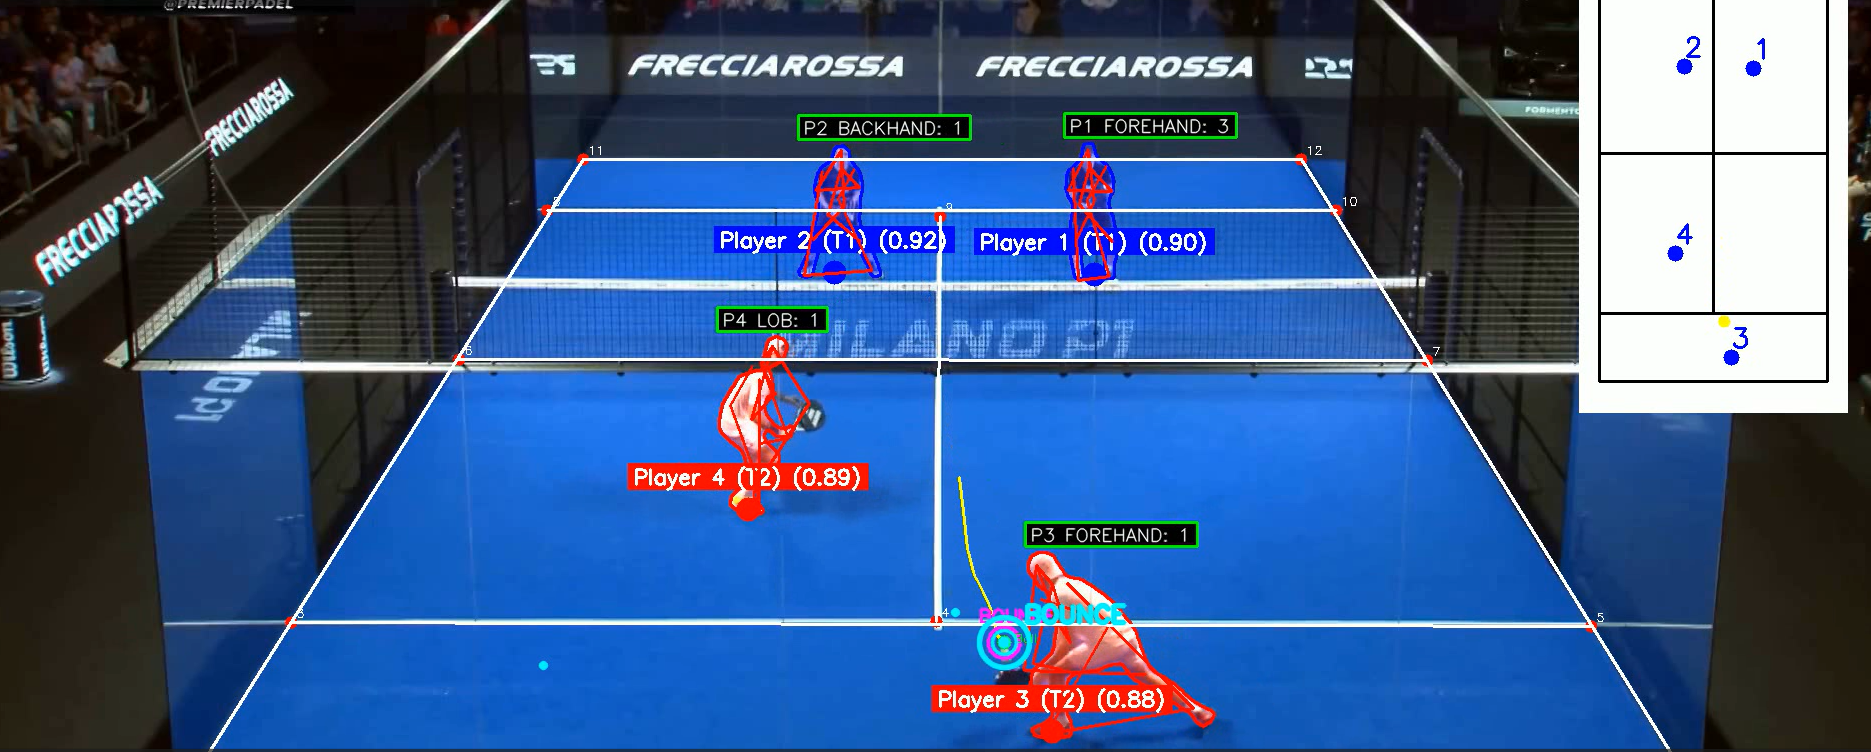
\includegraphics[width=0.85\textwidth]{figures/bounce_detection.png}
    \caption{Détection automatique d’un rebond à partir de l’analyse de la trajectoire de la balle.}
    \label{fig:bounce_detection}
\end{figure}
Pour être validé comme un véritable rebond et non comme un artefact de
prédiction, un pic détecté doit satisfaire deux critères
complémentaires~:
 
\begin{itemize}[leftmargin=*, itemsep=4pt]
 
    \item \textbf{Proéminence minimale}~: le pic doit se détacher de son
    voisinage immédiat d'au moins \textbf{4 pixels} de proéminence
    (\textit{prominence}). Ce seuil permet d'éliminer les faux maxima
    générés par les micro-oscillations résiduelles du signal de
    prédiction, qui peuvent faire trembler la position détectée de un à
    deux pixels d'une trame à l'autre sans correspondre à un événement
    physique réel.
 
    \item \textbf{Intervalle temporel minimal}~: deux rebonds consécutifs
    doivent être séparés d'au moins \textbf{0{,}45 seconde}, afin
    d'éviter les détections multiples issues d'un même contact avec le
    sol.
 
\end{itemize}
 
Cette double contrainte --- proéminence et distance temporelle --- confère
à la détection des rebonds une robustesse notable face au bruit
algorithmique inhérent aux prédictions par réseau de neurones.
 
\subsection{Sorties finales du module BallTracker}

Le module \textit{BallTracker} produit en sortie les indicateurs analytiques suivants :

\begin{itemize}
    \item La trajectoire spatio-temporelle complète de la balle, représentée par les coordonnées $(X, Y)$, le temps $t$ ainsi que l’état de visibilité.
    
    \item Les instants et positions des rebonds validés après le processus de filtrage et d’analyse de proéminence.
    
    \item La vitesse instantanée de la balle, estimée par différentiation temporelle des segments de trajectoire filtrés.
    
\end{itemize}
\begin{figure}[H]
    \centering
    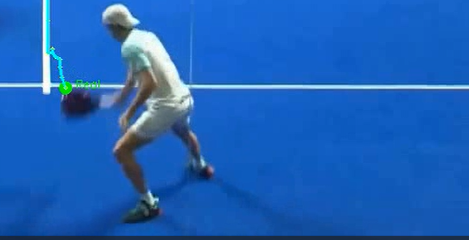
\includegraphics[width=0.32\textwidth]{figures/frame1.png}
    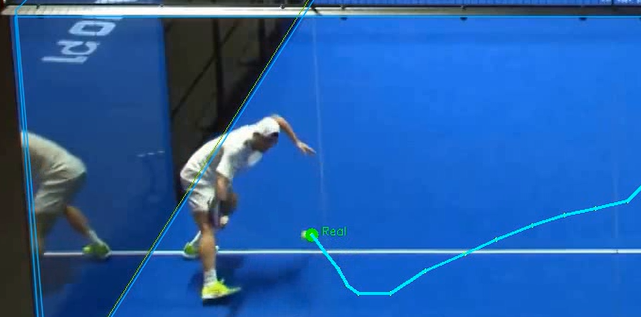
\includegraphics[width=0.32\textwidth]{figures/frame2.png}
    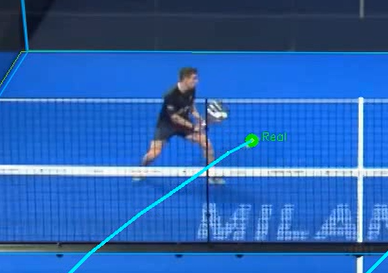
\includegraphics[width=0.32\textwidth]{figures/frame3.png}
    \caption{Illustrations de la position de la balle à différents instants.}
    \label{fig:ball_sequence}
\end{figure}
\subsubsection{Métriques d'évaluation et performances}

L'évaluation quantitative du système de suivi de la balle a été réalisée sur notre base de données de test à l'aide de deux métriques académiques de référence :

\begin{enumerate}
    \item \textbf{PCK@5px (Percentage of Correct Keypoints) :} Pourcentage de prédictions dont la distance euclidienne à la vérité terrain est inférieure ou égale à $5$~pixels.
    \item \textbf{RMSE (Root Mean Squared Error) :} Erreur quadratique moyenne globale en pixels sur l'ensemble de la trajectoire.
\end{enumerate}

Afin de mesurer l'impact de notre chaîne de post-traitement physique et géométrique, nous comparons les performances du modèle \textbf{TrackNet brut} avec notre \textbf{pipeline de suivi robuste} :

\begin{table}[h]
    \centering
    \caption{Comparaison des performances avant et après post-traitement}
    \label{tab:perf_posttraitement}

    \begin{tabular}{lcc}
        \toprule
        \textbf{Configuration} & \textbf{PCK @ 5px ($\uparrow$)} & \textbf{RMSE (pixels) ($\downarrow$)} \\
        \midrule
        \textbf{TrackNet (Brut)} & 86,5 \% & 4,82 px \\
        
        \textbf{Tracknet + les filtres} & \textbf{96,2 \%} & \textbf{1,78 px} \\
        \bottomrule
    \end{tabular}
\end{table}

\textbf{Analyse des résultats :} L'introduction du filtrage robuste permet un gain de \textbf{+9,7 \%} sur le PCK et une division par plus de 2,5 de l'erreur moyenne de trajectoire (RMSE passant de 4,82 à 1,78 pixels). Cette amélioration s'explique par l'élimination systématique des reflets vitrés par le filtre de vitesse et de marge, couplée à la reconstruction fluide des trajectoires d'occlusion par l'interpolation parabolique.

\subsection{Précision, rappel et score F1}

Ces métriques évaluent la capacité du réseau à détecter la présence de la balle sans générer de faux positifs.

\begin{table}[h]
    \centering
    \caption{Comparaison des performances des modèles TrackNet}
    \label{tab:perf_tracknet}
    \vspace{0.5em}
    \begin{tabular}{lccc}
        \toprule
        \textbf{Modèle} & \textbf{Précision} & \textbf{Rappel (Recall)} & \textbf{Score F1} \\
        \midrule
        \textbf{TrackNet (V1)} & 99,7 \% & 97,3 \% & 98,5 \% \\
        \textbf{TrackNetV2}    & 99,6 \% & 94,5 \% & 97,0 \% \\
        \textbf{GridTrackNet}  & 96,6 \% & 93,9 \% & 95,3 \% \\
        \textbf{TrackNetV3}    & 97,8 \%& 99,3 \% & 98,6 \% \\
        \textbf{TrackNetV4}    & 99,6 \% & 92,2 \% & 95,8 \% \\
        \textbf{TrackNetV5}    & 99,2 \% & 98,0 \% & 98,6 \% \\
        \bottomrule
    \end{tabular}
\end{table}

\subsection{Perspectives d'amélioration}

Pour les futures itérations du système, deux axes principaux d’amélioration sont envisagés :

\begin{itemize}
    \item \textbf{Estimation du fond (\textit{Background Estimation}) :} intégrer une image médiane du terrain comme donnée auxiliaire afin d’aider le modèle à distinguer la balle des distractions visuelles telles que les spectateurs ou les panneaux publicitaires.
    
    \item \textbf{Reconstruction 3D :} exploiter les trajectoires 2D détectées afin de reconstruire une représentation tridimensionnelle de la balle, permettant une analyse plus précise de la hauteur et de la vitesse indépendamment de la perspective de la caméra.
\end{itemize}
 
% ------------------------------------------------------------------
\subsection{Synthèse}
\label{subsec:synthesis}
% ------------------------------------------------------------------
 
Le module de suivi de balle repose sur une architecture hybride
combinant la puissance de représentation des réseaux convolutifs
temporels avec une chaîne de post-traitement physiquement informée.
L'intégration de TrackNet pour la génération de heatmaps, couplée à
l'inférence de visibilité, à l'ensemble temporel et au filtrage
multi-étapes, permet d'obtenir une trajectoire de balle précise, continue
et robuste, même dans des conditions visuelles difficiles telles que les
occlusions par les joueurs, les réflexions sur parois vitrées ou les
passages hors-champ. Ces caractéristiques en font un composant central
et fiable du système d'analyse sportive développé dans ce projet.

% ─────────────────────────────────────────────────────────────
\section{Suivi des joueurs}
% ─────────────────────────────────────────────────────────────
 
\subsection{Vue d'ensemble et positionnement dans le pipeline}
 
Le suivi des joueurs produit, à chaque frame, une représentation stable
de la position et de l'identité des quatre joueurs.
Cette stabilité est indispensable aux analyses aval : sans identifiants
persistants, il est impossible de calculer des trajectoires, d'attribuer
des frappes ou de distinguer les deux équipes.
 
Le module adopte une architecture en pipeline séquentiel, de la vidéo
brute jusqu'à la représentation structurée des joueurs, dont les
étapes sont décrites dans les sections suivantes.

 \begin{figure}[H]
    \centering
    \maybeincludegraphics[width=0.9\textwidth]{images_chap2/pipeline_joueurs.png}
    \caption{Pipeline de suivi des joueurs et modules d'identification des équipes.}
    \label{fig:pipeline_joueurs}
\end{figure}
% ─────────────────────────────────────────────────────────────
\subsection{Conversion BGR \texorpdfstring{$\rightarrow$}{->} RGB}
 
Avant toute opération de détection, chaque frame est convertie de
l'espace colorimétrique BGR (format natif d'OpenCV) vers RGB.
Cette conversion est requise car YOLO26 a été entraîné sur des images
en format RGB ; l'omettre introduirait un décalage colorimétrique
systématique dégradant les performances de détection et la cohérence
des descripteurs d'apparence extraits en aval.
 
% ─────────────────────────────────────────────────────────────
\subsection{Détection par YOLO26 fine-tuné}
 
\subsubsection{Choix du modèle YOLO26}
 
Le choix de YOLO26 résulte d'une comparaison entre plusieurs
architectures de détection.
Les modèles de petite taille (nano, small) offrent une vitesse
supérieure mais une précision insuffisante pour des silhouettes filmées
à 15--20\,m de hauteur.
Les modèles larges sont trop coûteux pour un déploiement en temps réel.
L'architecture medium constitue le meilleur compromis
précision/vitesse.
Par rapport aux détecteurs génériques, YOLO26 bénéficie d'un
fine-tuning spécifique sur des images de padel en vue aérienne
(26\textsuperscript{ème} cycle d'entraînement), lui conférant une
robustesse accrue aux silhouettes de faible résolution, aux angles de
vue atypiques et aux occlusions fréquentes entre joueurs.
 
% À insérer dans votre préambule (avant \begin{document}) si ce n'est pas déjà fait :
% \usepackage{tabularx}
% \usepackage{booktabs}

\subsubsection{Paramètres d'inférence}

\begin{table}[h]
    \centering
    \caption{Paramètres d'inférence du détecteur YOLO pour la localisation des joueurs}
    \vspace{0.5em}
    \begin{tabular}{l c p{6.5cm}}
        \toprule
        \textbf{Paramètre} & \textbf{Valeur} & \textbf{Objectif / Justification} \\
        \midrule
        \textbf{Seuil de confiance}  & 0,5 & Élimination des détections ambiguës et faux positifs \\
        \textbf{Seuil IoU (NMS)}     & 0,7 & Suppression des détections redondantes (joueur unique) \\
        \textbf{Résolution d'entrée} & 1280 px & Lisibilité des silhouettes filmées en vue aérienne \\
        \textbf{Classe cible}        & Personne & Restriction exclusive à la détection humaine \\
        \bottomrule
    \end{tabular}
    \label{tab:yolo_params}
\end{table}
 
La résolution de 1280\,px a été retenue pour préserver la lisibilité des
silhouettes filmées à 15--20\,m de hauteur : à plus basse résolution, ces
cibles de faible taille apparente deviennent difficiles à localiser de
manière fiable.
 
\subsubsection{Traitement en lot}
 
Les images sont regroupées en lots de quatre pour une seule passe
\textit{forward}, atteignant un débit environ 3,5$\times$ supérieur
au traitement image par image.
Le dernier lot incomplet en fin de vidéo est géré explicitement.
 
% ─────────────────────────────────────────────────────────────
\begin{figure}[H]
    \centering
    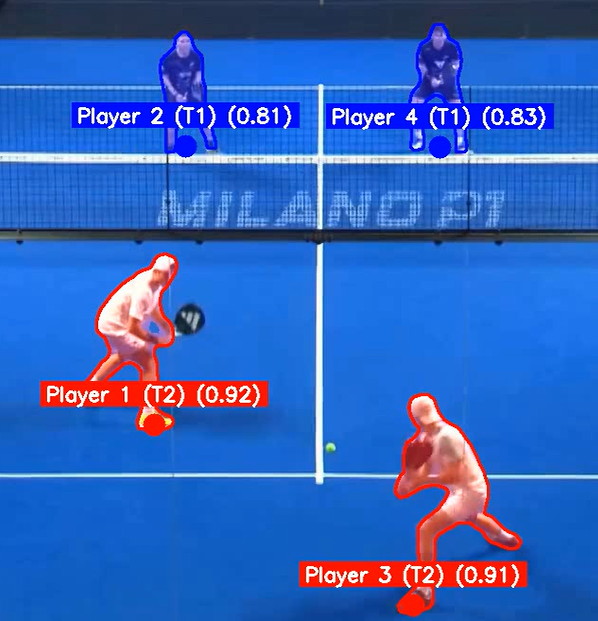
\includegraphics[width=0.79\textwidth]{figures/player_detection_result.png}
    \caption{Résultat du module de détection des joueurs. Chaque joueur est détecté par le modèle YOLO et associé à une équipe (T1 ou T2) ainsi qu'à un score de confiance. Les masques de segmentation permettent une localisation précise des joueurs sur le terrain.}
    \label{fig:player_detection_result}
\end{figure}
\subsection{Filtrage spatial par zone polygonale}
 
\subsubsection{Définition du polygone de terrain}
 
La détection brute génère des faux positifs extérieurs au terrain
(spectateurs, arbitres, cameramen).
Un filtre géométrique appliqué en sortie du détecteur les élimine.
Le terrain est modélisé par 12 points clés définis à la calibration ;
le polygone de filtrage est délimité par les quatre coins extérieurs
\textbf{k1}, \textbf{k2}, \textbf{k12} et \textbf{k11}.

\begin{figure}[H]
    \centering
    \maybeincludegraphics[width=0.9\textwidth]{images_chap2/figure_terrain (1).png}
    \caption{Représentation schématique du terrain de padel avec la zone de filtrage polygonale.}
    \label{fig:terrain_filtrage}
\end{figure}
 
 
\subsubsection{Test d'appartenance à la zone de jeu}
 
L'appartenance est déterminée par un test point-dans-polygone
(\textit{ray-casting}) appliqué au centre-bas de chaque boîte
englobante (point correspondant aux pieds du joueur).
Seules les détections dont le point au sol est à l'intérieur du
quadrilatère sont conservées~--- en pratique, les quatre joueurs
actifs par image.
 
% ─────────────────────────────────────────────────────────────
\subsubsection{Association et suivi : algorithme d’identité stable}

Contrairement aux approches de suivi classiques telles que \textit{ByteTrack}, qui peuvent engendrer des dérives ou des permutations d’identifiants (\textit{ID switches}) lors d’occlusions prolongées ou de croisements à proximité du filet, la stratégie adoptée dans ce module repose sur une identité verrouillée. Une fois les quatre identifiants de joueurs attribués durant la phase d’initialisation, ils demeurent constants tout au long de la séquence vidéo.

\paragraph{Initialisation et assignation des équipes}

La phase d’initialisation est déclenchée de manière déterministe dès que le détecteur observe exactement quatre joueurs simultanément à l’intérieur du polygone représentant le terrain. Les détections sont alors triées selon leur coordonnée verticale $y$ croissante (du haut vers le bas de l’image, ce qui correspond à l’éloignement de la caméra). Les identifiants stables de 1 à 4 sont ensuite attribués définitivement.

L’appartenance à une équipe est déduite directement de cette organisation spatiale lors de la première image valide :

\begin{itemize}
    \item \textbf{Équipe A (Team 1)} : composée des joueurs 1 et 2, correspondant aux deux plus faibles valeurs de $y$, situés dans la moitié supérieure de l’image.
    \item \textbf{Équipe B (Team 2)} : composée des joueurs 3 et 4, correspondant aux deux plus grandes valeurs de $y$, situés dans la moitié inférieure de l’image.
\end{itemize}

Cette stratégie d’initialisation élimine l’instabilité liée à un regroupement (\textit{clustering}) initial et garantit des statistiques d’équipe cohérentes dès les premières images.

\paragraph{Extraction du descripteur d’apparence}

Afin de caractériser visuellement chaque joueur, le système extrait un descripteur de couleur RGB calculé sur les 40\,\% supérieurs de la boîte englobante, correspondant principalement au torse et au maillot. Pour réduire le bruit lié aux plis du tissu et aux variations de texture, un filtre gaussien bidimensionnel de taille $5 \times 5$ est appliqué à la région extraite avant le calcul de la moyenne des canaux :

\[
e = \frac{1}{|\Omega|} \sum_{(r,g,b)\in\Omega}(r,g,b)
\tag{2.4}
\]

où $\Omega$ désigne l’ensemble des pixels de la région considérée.

Le vecteur tridimensionnel
\[
e = [R_{\text{moy}}, G_{\text{moy}}, B_{\text{moy}}]
\]
constitue une signature d’apparence légère permettant de différencier les joueurs, notamment lors des croisements rapprochés.

\paragraph{Prédiction cinématique}

Avant l’étape d’association temporelle, la position future de chaque piste active est estimée par extrapolation linéaire en ajoutant à la position courante une vitesse lissée par une moyenne mobile exponentielle (EMA) avec $\alpha_v = 0{,}5$ :

\[
\hat{b}_{t+1} = b_t + v_t
\tag{2.5}
\]

La vitesse instantanée $v_{\text{inst}}$ est calculée à partir de la différence entre les centres courant et précédent de la boîte englobante. Afin de garantir la cohérence physique du mouvement, le système vérifie que le centre de la boîte prédite $\hat{b}_{t+1}$ demeure à l’intérieur du polygone du terrain. Si ce point sort des limites, la vitesse de la piste est immédiatement réinitialisée à zéro et la prédiction est figée sur la dernière position valide, évitant ainsi toute dérive.

\paragraph{Matrice de coûts et algorithme Hongrois}

L’association entre les pistes actives prédites et les nouvelles détections de l’image courante est formulée comme un problème d’affectation linéaire optimale. Le coût d’association $C(r,c)$ entre une piste $r$ et une détection $c$ est défini par :

\[
C(r,c)=
\begin{cases}
10\,000, & \text{si } d_{\text{spatial}} > 300 \text{ px} \\
d_{\text{spatial}} + 200 \cdot d_{\text{couleur}} + 5 \cdot missed_r, & \text{sinon}
\end{cases}
\tag{2.6}
\]

où :

\begin{itemize}
    \item $d_{\text{spatial}} = \|\hat{c}_r - c_c\|_2$ est la distance euclidienne (en pixels) entre le centre prédit $\hat{c}_r$ de la piste $r$ et le centre $c_c$ de la détection $c$.
    \item $d_{\text{couleur}} = \dfrac{\|e_r - e_c\|_2}{255}$ est la distance euclidienne normalisée entre les signatures colorimétriques.
    \item $missed_r$ représente le nombre d’images consécutives durant lesquelles la piste $r$ n’a pas été associée à une détection.
\end{itemize}

Le seuil géométrique strict de 300 pixels agit comme une étape de \textit{gating}, attribuant un coût prohibitif de 10\,000 à toute association jugée physiquement impossible. Le coefficient 200 appliqué à la distance colorimétrique confère un poids important à l’identité visuelle du maillot.

La résolution globale de cette matrice de coûts est assurée par l’algorithme de Kuhn-Munkres, également appelé algorithme Hongrois, dont la complexité est de $\mathcal{O}(n^3)$.

\paragraph{Mise à jour des pistes par moyenne exponentielle mobile}

Une fois l’association résolue, les états des pistes ayant trouvé une correspondance sont mis à jour comme suit :

\begin{itemize}
    \item \textbf{Vitesse :} si le joueur a été absent durant plus de cinq images ($missed > 5$), sa vitesse est réinitialisée à zéro. Sinon, elle est mise à jour à l’aide d’une EMA réactive ($\alpha_v = 0{,}5$) :
    \[
    v_t \leftarrow 0.5 \cdot v_{\text{inst}} + 0.5 \cdot v_{t-1}
    \]

    \item \textbf{Apparence :} le descripteur colorimétrique est actualisé à l’aide d’une EMA à mémoire longue ($\alpha_c = 0{,}1$), permettant de s’adapter progressivement aux variations d’éclairage :
    \[
    e_t \leftarrow 0.1 \cdot e_{\text{det}} + 0.9 \cdot e_{t-1}
    \]
\end{itemize}

Cette combinaison entre prédiction cinématique, descripteur d’apparence et association globale garantit un suivi robuste et stable des quatre joueurs sur l’ensemble de la vidéo, tout en éliminant efficacement les permutations d’identifiants.

% ─────────────────────────────────────────────────────────────
\subsection{Robustesse aux situations critiques}
 
\subsubsection{Occlusion et croisement de joueurs}
 
Lors d'un croisement, les boîtes englobantes deviennent
quasi-identiques spatialement.
L'algorithme Hongrois minimise le coût global de l'affectation plutôt
que paire par paire, identifiant la combinaison optimale.
Le descripteur colorimétrique joue alors un rôle discriminant essentiel
entre joueurs d'équipes différentes.
 
\subsubsection{Disparition temporaire d'un joueur}
 
Un joueur absent (sortie de terrain, occlusion totale, chute) voit son
identifiant maintenu pendant 90 frames ($\approx$3\,s à 30\,fps), sa
position extrapolée à partir de sa dernière vitesse.
Au-delà de 5 frames d'absence, la vitesse est réinitialisée à zéro
pour éviter une extrapolation divergente.
Passé le délai de 90 frames sans réassociation, la piste est supprimée
et un nouveau cycle d'initialisation est attendu.
La pénalité progressive garantit une récupération rapide dès la
réapparition du joueur.
 
\subsubsection{Nombre insuffisant de joueurs détectés}
 
En phase d'initialisation, si le nombre de détections est différent de
quatre, le système diffère d'une frame sans produire de sortie.
En phase de suivi active, les pistes établies sont maintenues par le
mécanisme de persistance prédictive.
 
% ─────────────────────────────────────────────────────────────
\subsection{Extension par segmentation au niveau pixel}
 
Une variante intègre SAM2 (\textit{Segment Anything Model 2}) en
complément de YOLO26 : les boîtes englobantes servent de
\textit{prompts} au modèle de segmentation, qui produit des masques
pixel-level.
Cette extension améliore la précision de localisation pour des analyses
de posture ou de gestuelle, au prix d'un coût computationnel nettement
plus élevé, réservé aux scénarios où la précision prime sur le temps
réel.
 
% ─────────────────────────────────────────────────────────────
\subsection{Synthèse}
Le module de suivi des joueurs repose sur un enchaînement séquentiel de cinq étapes clés :
\begin{enumerate}
    \item \textbf{Prétraitement colorimétrique :} La conversion de l'espace $BGR \rightarrow RGB$ afin d'éviter tout décalage colorimétrique lors de l'inférence et de l'extraction des signatures.
    \item \textbf{Détection et filtrage spatial :} L'inférence par le modèle YOLO26 fine-tuné à haute résolution ($1280$~px) couplée à un filtrage géométrique par lancer de rayon (\textit{ray-casting}) dans le polygone convexe défini par les limites du court.
    \item \textbf{Partitionnement géographique initial :} L'attribution déterministe des équipes lors du premier frame valide (moitié supérieure pour l'équipe A, moitié inférieure pour l'équipe B), évitant l'instabilité des méthodes de clustering non supervisées au démarrage.
    \item \textbf{Association globale optimale :} L'appariement des pistes et des détections via l'algorithme Hongrois, en minimisant une matrice de coûts composite associant distance euclidienne spatiale, distance colorimétrique RGB du torse et pénalité de disparition temporelle.
    \item \textbf{Gestion robuste des occlusions :} La persistance prédictive des pistes par extrapolation cinématique et maintien de la mémoire couleur (\textit{slot-holding}) jusqu'à $90$~frames (environ $3$~secondes à $30$~fps).
\end{enumerate}

Cet ensemble de mécanismes garantit un suivi stable et continu sur toute la durée du match, ce qui constitue une condition \textit{sine qua non} pour la fiabilité des modules d'analyse statistique situés en aval du pipeline.


\section{Modèle d'estimation des points clés des joueurs}

\subsection{Introduction}

La détection des joueurs par boîtes englobantes permet uniquement de localiser les athlètes dans l’image. Cependant, cette représentation reste insuffisante pour analyser précisément les mouvements, les postures et les gestes techniques durant un match de padel.

Afin d’obtenir une compréhension plus détaillée des actions des joueurs, la plateforme SmartPlayAI intègre un module d’estimation de pose basé sur YOLOv8-Pose. Ce modèle permet d’extraire automatiquement les points clés squelettiques des joueurs à partir des séquences vidéo et de représenter leur posture en temps réel.

\subsection{Architecture du modèle YOLOv8-Pose}

Le modèle utilisé repose sur l’architecture YOLOv8-Pose, capable d’effectuer simultanément la détection des joueurs et l’estimation de leurs points clés dans une seule passe d’inférence. Cette approche améliore considérablement les performances temps réel.

L’architecture comprend trois composants principaux :

\begin{itemize}
    \item \textbf{Backbone (CSPDarknet)} : extraction des caractéristiques visuelles profondes ;
    \item \textbf{Neck (PAN-FPN)} : fusion multi-échelles des cartes de caractéristiques ;
    \item \textbf{Pose Head} : prédiction des boîtes englobantes et des points clés corporels.
\end{itemize}

\begin{table}[H]
\centering
\caption{Composants principaux de YOLOv8-Pose}
\label{tab:composants_yolopose}
\begin{tabular}{|c|c|}
\hline
\textbf{Composant} & \textbf{Rôle} \\
\hline
Backbone & Extraction des caractéristiques visuelles \\
\hline
Neck & Fusion multi-échelles \\
\hline
Pose Head & Prédiction des keypoints et des boîtes \\
\hline
\end{tabular}
\end{table}

\subsection{Estimation des points clés}

Pour chaque joueur détecté, le modèle prédit les coordonnées des articulations corporelles selon la convention COCO à 17 points clés. Chaque articulation est représentée par :

\begin{equation}
p_i = (x_i, y_i, c_i)
\end{equation}

où :
\begin{itemize}
    \item $x_i$ et $y_i$ représentent les coordonnées du point clé ;
    \item $c_i$ correspond au score de confiance associé.
\end{itemize}

Les points clés couvrent les principales régions anatomiques : tête, épaules, coudes, poignets, hanches, genoux et chevilles.

\subsection{Pipeline d’inférence}

Le traitement d’une trame vidéo commence par une phase de prétraitement et de normalisation de l’image d’entrée. Les caractéristiques visuelles profondes sont ensuite extraites à l’aide du Backbone, puis fusionnées à différentes échelles grâce au module Neck afin d’améliorer la détection des structures anatomiques. Le modèle réalise ensuite la détection des joueurs ainsi que l’estimation simultanée des points clés corporels. Les détections redondantes sont supprimées à l’aide de l’algorithme NMS (\textit{Non-Maximum Suppression}), avant de générer les squelettes associés aux joueurs détectés. Cette pipeline permet d’obtenir en temps réel une représentation squelettique complète et précise des joueurs présents sur le terrain.

\subsection{Adaptation au contexte du padel}

L’estimation de pose dans le padel reste complexe à cause des mouvements rapides, des occultations et des vues aériennes. Afin d’améliorer les performances, un fine-tuning du modèle a été réalisé sur des séquences réelles de matchs de padel.

Cette adaptation permet d’augmenter la précision des articulations détectées et d’améliorer la robustesse du système dans des scènes sportives dynamiques.

\subsection{Applications dans SmartPlayAI}

Les points clés extraits sont exploités dans plusieurs modules analytiques :

\begin{table}[H]
\centering
\caption{Applications des points clés dans SmartPlayAI}
\label{tab:applications_keypoints}
\begin{tabular}{|c|c|}
\hline
\textbf{Application} & \textbf{Utilité} \\
\hline
Projection géométrique & Position précise des joueurs sur le terrain \\
\hline
Reconnaissance de gestes & Détection des smashs, volées et revers \\
\hline
Analyse biomécanique & Étude des angles articulaires et des mouvements \\
\hline
\end{tabular}
\end{table}

Les données squelettiques permettent ainsi d’enrichir l’analyse tactique et biomécanique des matchs.

\subsection{Conclusion}

Le module YOLOv8-Pose constitue un élément essentiel de SmartPlayAI. Grâce à l’estimation des points clés, le système dépasse la simple détection des joueurs et fournit une analyse avancée des mouvements, des gestes techniques et des comportements tactiques durant les matchs de padel.
% ════════════════════════════════════════════════════════════════════════════
\section{Module d'analyse biomécanique et tactique}
% ════════════════════════════════════════════════════════════════════════════

\subsection{Objectifs et rôle du module}

Le module d'analyse biomécanique et tactique constitue le noyau analytique de la plateforme
SmartPlayAI. Son rôle fondamental est de transformer les coordonnées brutes des joueurs et de
la balle — issues de la chaîne de détection et de suivi vidéo — en un ensemble structuré
d'indicateurs quantitatifs exploitables à des fins d'analyse de la performance sportive.

À partir des positions projetées dans le référentiel métrique du terrain, le module calcule
un ensemble d'indicateurs cinématiques couvrant les déplacements, les vitesses, les
accélérations et les distances parcourues. Ces grandeurs servent ensuite à identifier les
événements de jeu, à caractériser les actions techniques réalisées par les joueurs et à
alimenter un système automatisé de suivi du score.

Ce module assure ainsi la transition entre les données brutes issues de la vision par
ordinateur et les informations à forte valeur ajoutée destinées aux entraîneurs, aux
analystes et aux joueurs. Ses objectifs principaux se déclinent en quatre axes :

\begin{itemize}[leftmargin=1.5em]
  \item Projection et normalisation spatiale des positions détectées dans un référentiel
        métrique standardisé ;
  \item Construction d'un modèle de données temporel enrichi regroupant déplacements,
        vitesses et accélérations à plusieurs granularités temporelles ;
  \item Détection et classification automatique des événements de jeu (frappes, types
        de coups) ;
  \item Suivi automatisé du score conformément aux règles officielles du padel.
\end{itemize}

% ────────────────────────────────────────────────────────────────────────────
\subsection{Architecture générale du pipeline d'analyse}
% ────────────────────────────────────────────────────────────────────────────

Le pipeline d'analyse repose sur une succession d'étapes permettant d'enrichir
progressivement les données extraites de la vidéo. Chaque étape produit une représentation
plus élaborée de l'information, depuis les coordonnées pixel brutes jusqu'à un ensemble
complet d'indicateurs analytiques prêts à l'exportation.

Dans un premier temps, les positions des joueurs et de la balle sont exprimées dans un
référentiel métrique associé au terrain de padel. Ces positions sont ensuite organisées
sous la forme d'une structure de données temporelle permettant de suivre l'évolution de
chaque entité au cours du match. Les données ainsi structurées servent ensuite au calcul
des indicateurs biomécaniques, lesquels alimentent en aval les modules de détection des
frappes, de reconnaissance des types de coups et de mise à jour automatique du score.

Le Tableau~\ref{tab:pipeline_dataanalytics} résume les six étapes séquentielles du pipeline
ainsi que les formats de données produits à chaque niveau de traitement.

\begin{table}[H]
  \centering
  \renewcommand{\arraystretch}{1.3}
  \begin{tabularx}{\textwidth}{L{2.8cm} X L{4cm}}
    \rowcolor{tablehead}
    \textcolor{white}{\textbf{Étape}} &
    \textcolor{white}{\textbf{Description}} &
    \textcolor{white}{\textbf{Format de sortie}} \\
    \rowcolor{rowalt}
    Acquisition   & Réception des positions des joueurs et de la balle à chaque trame vidéo
                  & Coordonnées pixel $(p_x, p_y)$ \\
    Projection    & Transformation homographique et conversion en unités métriques
                  & Coordonnées métriques $(x_m, y_m)$ \\
    \rowcolor{rowalt}
    Accumulation  & Construction d'un enregistrement par trame et empilement en série temporelle
                  & Liste de $N$ enregistrements \\
    Enrichissement & Calcul des déplacements, vitesses et accélérations sur 4 intervalles temporels
                  & DataFrame de 179 colonnes \\
    \rowcolor{rowalt}
    Analyse événementielle & Détection des frappes, classification des coups, suivi du score
                  & Événements horodatés + score \\
    Export        & Sérialisation en fichier CSV pour exploitation post-match
                  & Fichier \texttt{.csv} ($\approx 3{,}2$\,Mo/match) \\
  \end{tabularx}
  \caption{Flux de traitement du module DataAnalytics}
  \label{tab:pipeline_dataanalytics}
\end{table}

% ────────────────────────────────────────────────────────────────────────────
\subsection{Acquisition et structuration des données}
% ────────────────────────────────────────────────────────────────────────────

\subsubsection{Référentiel spatial du terrain}

L'ensemble des calculs est réalisé dans un système de coordonnées métrique centré sur le
filet. Ce choix garantit une symétrie naturelle entre les deux demi-terrains et simplifie
les comparaisons entre équipes. Les dimensions réglementaires définies par la Fédération
Internationale de Padel (FIP) fixent les bornes du référentiel :

\begin{itemize}[leftmargin=1.5em]
  \item L'axe $X$ (largeur du terrain) s'étend de $-5$\,m à $+5$\,m ;
  \item L'axe $Y$ (longueur du terrain) s'étend de $-10$\,m à $+10$\,m.
\end{itemize}

Le Tableau~\ref{tab:constantes_fip} récapitule les constantes réglementaires FIP utilisées
pour définir les bornes du référentiel.

\begin{table}[H]
  \centering
  \renewcommand{\arraystretch}{1.3}
  \begin{tabularx}{\textwidth}{L{4.4cm} C{2cm} C{1.5cm} X}
    \rowcolor{tablehead}
    \textcolor{white}{\textbf{Constante}} &
    \textcolor{white}{\textbf{Valeur}} &
    \textcolor{white}{\textbf{Axe}} &
    \textcolor{white}{\textbf{Description}} \\
    \rowcolor{rowalt}
    \texttt{base\_line}         & 10\,m & $X$ & Demi-largeur du terrain \\
    \texttt{side\_line}         & 20\,m & $Y$ & Longueur totale du terrain \\
    \rowcolor{rowalt}
    \texttt{service\_side\_line} & 3\,m  & $Y$ & Distance ligne de service au fond de court \\
    \texttt{net\_side\_line}    & 10\,m & $Y$ & Distance filet au fond de court \\
  \end{tabularx}
  \caption{Constantes réglementaires FIP et bornes du référentiel terrain}
  \label{tab:constantes_fip}
\end{table}

\subsubsection{Projection homographique des positions}

La caméra placée en vue aérienne capture le terrain selon une perspective introduisant des
déformations géométriques. Pour corriger ces distorsions et obtenir des coordonnées métriques
fidèles, une transformation homographique est appliquée — représentation mathématique standard
d'une projection plan-à-plan en vision par ordinateur.

Formellement, un point $\mathbf{p} = (p_x, p_y)^\top$ exprimé en pixels est converti en
coordonnées homogènes $\tilde{\mathbf{p}} = (p_x, p_y, 1)^\top$, puis projeté par la matrice
d'homographie $H \in \mathbb{R}^{3 \times 3}$ calculée lors de l'étalonnage de la caméra :

\begin{equation}
  \tilde{\mathbf{p}}' = H \cdot \tilde{\mathbf{p}}, \qquad
  \mathbf{p}' = \frac{1}{\tilde{p}'_3} \cdot \bigl(\tilde{p}'_1,\, \tilde{p}'_2\bigr)^\top
  \label{eq:homographie}
\end{equation}

La conversion vers le référentiel métrique FIP s'effectue ensuite en soustrayant l'origine
(centre du filet) et en appliquant les facteurs d'échelle correspondant aux dimensions
réglementaires :

\begin{equation}
  x_m = \Delta p_x \cdot \frac{B_{\mathrm{LINE}}}{W_{\mathrm{terrain}}}, \qquad
  y_m = \Delta p_y \cdot \frac{S_{\mathrm{LINE}}}{H_{\mathrm{terrain}}}
  \label{eq:conversion_metrique}
\end{equation}

où $\Delta p_x$ et $\Delta p_y$ désignent les déplacements par rapport à l'origine dans la
mini-carte, et $W_{\mathrm{terrain}}$, $H_{\mathrm{terrain}}$ sont les dimensions en pixels
de cette mini-carte. On obtient ainsi, pour chaque joueur, une position $(x_m, y_m)$
exprimée en mètres dans le référentiel centré sur le filet.

\subsubsection{Structuration temporelle des observations}

À chaque trame vidéo, le système constitue un enregistrement structuré regroupant l'ensemble
des informations spatiales de l'instant considéré. Cet enregistrement comprend : l'indice de
trame (identifiant entier incrémental), la liste des positions des quatre joueurs exprimées en
coordonnées métriques, et la position de la balle (ou une valeur nulle si la balle n'est pas
détectée).

Ces enregistrements sont empilés au fil des trames pour constituer la série temporelle brute
qui alimente l'étape d'enrichissement cinématique. Cette organisation facilite l'analyse
dynamique des comportements individuels et collectifs au cours du match.

% ────────────────────────────────────────────────────────────────────────────
\subsection{Construction du modèle de données analytique}
% ────────────────────────────────────────────────────────────────────────────

L'ensemble des enregistrements accumulés est converti en un tableau de données tabulaire dont
chaque ligne correspond à une trame vidéo. Dans sa forme brute, ce tableau comporte 11 colonnes
de base décrites dans le Tableau~\ref{tab:colonnes_base}.

\begin{table}[H]
  \centering
  \renewcommand{\arraystretch}{1.3}
  \begin{tabularx}{\textwidth}{L{3.5cm} C{2cm} C{2cm} X}
    \rowcolor{tablehead}
    \textcolor{white}{\textbf{Colonne}} &
    \textcolor{white}{\textbf{Type}} &
    \textcolor{white}{\textbf{Unité}} &
    \textcolor{white}{\textbf{Description}} \\
    \rowcolor{rowalt}
    \texttt{frame}                        & entier & — & Indice de trame (0, 1, 2, \ldots) \\
    \texttt{player\{i\}\_x} ($i = 1..4$) & réel   & mètre & Position $X$ du joueur $i$ \\
    \rowcolor{rowalt}
    \texttt{player\{i\}\_y} ($i = 1..4$) & réel   & mètre & Position $Y$ du joueur $i$ \\
    \texttt{ball\_x}                      & réel   & mètre & Position $X$ de la balle \\
    \rowcolor{rowalt}
    \texttt{ball\_y}                      & réel   & mètre & Position $Y$ de la balle \\
  \end{tabularx}
  \caption{Colonnes de base du tableau de données brut}
  \label{tab:colonnes_base}
\end{table}

Chaque trame est associée à un horodatage absolu exprimé en secondes, calculé à partir de
l'indice de trame $n$ et de la cadence d'acquisition $f_s \in \{25, 30\}$ images par
seconde :

\begin{equation}
  t[n] = \frac{n}{f_s}
  \label{eq:horodatage}
\end{equation}

En ce qui concerne la gestion des données manquantes, lors des phases d'occultation (joueur
hors-champ, superposition de silhouettes), la détection peut échouer pour un ou plusieurs
joueurs. Ces absences sont enregistrées comme valeurs nulles puis converties en valeurs
indéfinies (\texttt{NaN}) lors de la construction du tableau. Ces valeurs manquantes sont
propagées de façon cohérente lors du calcul des indicateurs cinématiques, garantissant
qu'aucun artefact numérique n'est introduit dans les séries temporelles.

Enfin, la structure tabulaire unifiée ainsi constituée comporte 179 colonnes au total,
réparties en trois familles : 11 colonnes fixes (indices, horodatages, coordonnées),
4 colonnes temporelles (intervalles $\Delta t_k$) et 164 colonnes cinématiques issues de
l'enrichissement multi-intervalle décrit à la section suivante.

% ────────────────────────────────────────────────────────────────────────────
\subsection{Extraction des indicateurs biomécaniques}
% ────────────────────────────────────────────────────────────────────────────

L'enrichissement cinématique repose sur une stratégie multi-intervalle : les déplacements,
vitesses et accélérations sont calculés simultanément sur quatre fenêtres temporelles
correspondant à $k \in \{1, 2, 3, 4\}$ trames successives. L'intervalle temporel associé à
chaque valeur de $k$ est défini par :

\begin{equation}
  \Delta t_k[n] = t[n] - t[n-k] = \frac{k}{f_s}
  \label{eq:intervalle}
\end{equation}

Le Tableau~\ref{tab:niveaux_lissage} résume les quatre niveaux de lissage et leurs usages
recommandés. Le choix $k = 4$ (fenêtre de 133\,ms) est justifié par le fait que cette durée
correspond au seuil minimal du temps de réaction humain. Elle permet de réduire l'erreur de
bruit de position sans introduire de retard perceptible dans la détection des vrais
changements de direction.

\begin{table}[H]
  \centering
  \renewcommand{\arraystretch}{1.3}
  \begin{tabularx}{\textwidth}{C{1cm} C{2.5cm} C{2cm} X}
    \rowcolor{tablehead}
    \textcolor{white}{\textbf{$k$}} &
    \textcolor{white}{\textbf{$\Delta t_k$ à 30\,fps}} &
    \textcolor{white}{\textbf{Lissage}} &
    \textcolor{white}{\textbf{Usage recommandé}} \\
    \rowcolor{rowalt}
    1 & $\approx 33$\,ms  & Aucun   & Signal de référence ; bruit de détection élevé \\
    2 & $\approx 67$\,ms  & Faible  & Détection des changements dynamiques rapides \\
    \rowcolor{rowalt}
    3 & $\approx 100$\,ms & Modéré  & Analyse des transitions tactiques \\
    4 & $\approx 133$\,ms & Fort    & Recommandé — lissage optimal pour la performance \\
  \end{tabularx}
  \caption{Intervalles temporels et niveaux de lissage associés}
  \label{tab:niveaux_lissage}
\end{table}

\subsubsection{Analyse des déplacements}

Le déplacement entre la trame $n-k$ et la trame $n$ est calculé, pour chaque composante,
par différence arithmétique des positions :

\begin{equation}
  \Delta x_k[n] = x[n] - x[n-k], \qquad \Delta y_k[n] = y[n] - y[n-k]
  \label{eq:deplacement}
\end{equation}

Ces grandeurs sont exprimées en mètres. Pour $k = 4$ à 30\,fps, les plages typiques
observées en match de padel sont comprises entre $-30$\,cm et $+30$\,cm, reflétant les
micro-ajustements posturaux et les déplacements courts caractéristiques de ce sport.

\subsubsection{Analyse des vitesses}

La vitesse instantanée est estimée par différences finies du premier ordre appliquées aux
déplacements. Pour chacune des deux composantes :

\begin{equation}
  V_{x,k}[n] = \frac{\Delta x_k[n]}{\Delta t_k} = \frac{x[n] - x[n-k]}{k/f_s}
  \label{eq:vitesse_x}
\end{equation}

\begin{equation}
  V_{y,k}[n] = \frac{\Delta y_k[n]}{\Delta t_k}
  \label{eq:vitesse_y}
\end{equation}

La vitesse scalaire (norme euclidienne du vecteur vitesse) est définie par :

\begin{equation}
  V_{\mathrm{norm},k}[n] = \sqrt{V_{x,k}[n]^2 + V_{y,k}[n]^2}
  \label{eq:vitesse_norme}
\end{equation}

Le Tableau~\ref{tab:vitesses_padel} présente les plages de vitesse scalaire caractéristiques
observées en match de padel.

\begin{table}[H]
  \centering
  \renewcommand{\arraystretch}{1.3}
  \begin{tabularx}{\textwidth}{X C{3.5cm}}
    \rowcolor{tablehead}
    \textcolor{white}{\textbf{Situation locomotrice}} &
    \textcolor{white}{\textbf{$V_{\mathrm{norm}}$ (m/s)}} \\
    \rowcolor{rowalt}
    Joueur immobile (phase d'attente)    & $0{,}0 - 0{,}3$ \\
    Déplacement latéral (pas chassés)    & $1{,}5 - 3{,}5$ \\
    \rowcolor{rowalt}
    Sprint en direction d'un smash       & $4{,}0 - 6{,}5$ \\
    Vitesse maximale relevée             & $\approx 7{,}0$ \\
  \end{tabularx}
  \caption{Plages de vitesse scalaire caractéristiques observées en match de padel}
  \label{tab:vitesses_padel}
\end{table}

\subsubsection{Analyse des accélérations}

L'accélération est obtenue par différences finies du second ordre appliquées aux vecteurs
vitesse :

\begin{equation}
  A_{x,k}[n] = \frac{V_{x,k}[n] - V_{x,k}[n-k]}{\Delta t_k}
  \label{eq:accel_x}
\end{equation}

\begin{equation}
  A_{y,k}[n] = \frac{V_{y,k}[n] - V_{y,k}[n-k]}{\Delta t_k}
  \label{eq:accel_y}
\end{equation}

L'accélération scalaire correspondante est :

\begin{equation}
  A_{\mathrm{norm},k}[n] = \sqrt{A_{x,k}[n]^2 + A_{y,k}[n]^2}
  \label{eq:accel_norme}
\end{equation}

Le Tableau~\ref{tab:accelerations_padel} répertorie les plages caractéristiques selon les
événements biomécaniques observés en padel.

\begin{table}[H]
  \centering
  \renewcommand{\arraystretch}{1.3}
  \begin{tabularx}{\textwidth}{X C{3.5cm}}
    \rowcolor{tablehead}
    \textcolor{white}{\textbf{Événement biomécanique}} &
    \textcolor{white}{\textbf{$A_{\mathrm{norm}}$ (m/s²)}} \\
    \rowcolor{rowalt}
    Course en régime stabilisé                              & $0{,}0 - 2{,}0$ \\
    Changement de direction                                 & $5{,}0 - 12{,}0$ \\
    \rowcolor{rowalt}
    Départ de sprint                                        & $8{,}0 - 15{,}0$ \\
    Phase de frappe (bras, via points squelettiques)        & $> 20{,}0$ \\
  \end{tabularx}
  \caption{Plages d'accélération scalaire caractéristiques observées en padel}
  \label{tab:accelerations_padel}
\end{table}

\subsubsection{Distance parcourue et intensité de jeu}

La distance inter-trame est calculée avec $k = 1$ (trames consécutives), afin de minimiser
les erreurs de rectification liées aux trajectoires curvilignes :

\begin{equation}
  d[n] = \sqrt{\bigl(x[n] - x[n-1]\bigr)^2 + \bigl(y[n] - y[n-1]\bigr)^2}
  \label{eq:distance_intertrame}
\end{equation}

La distance totale parcourue sur une séquence de $N$ trames s'obtient par sommation
cumulative :

\begin{equation}
  D_{\mathrm{tot}} = \sum_{n=1}^{N} d[n]
  \label{eq:distance_totale}
\end{equation}

Les valeurs typiques observées se situent entre 50 et 200\,m pour un échange complet, selon
l'intensité et la durée du rallye. Combinée aux vitesses et aux accélérations, cette métrique
permet d'évaluer la charge physique associée aux différentes phases de jeu.

% ────────────────────────────────────────────────────────────────────────────
\subsection{Analyse événementielle des échanges}
% ────────────────────────────────────────────────────────────────────────────

\subsubsection{Détection des frappes}

La détection d'un impact raquette-balle repose sur une hypothèse physique fondamentale : une
frappe se traduit par une discontinuité brutale du vecteur vitesse de la balle, caractérisée
soit par un changement de direction marqué, soit par une variation soudaine de son énergie
cinétique. L'algorithme opère en deux phases successives.

Lors de la première phase, les vitesses pré- et post-impact sont estimées sur une fenêtre
glissante de $W = 5$ trames de part et d'autre du moment analysé :

\begin{equation}
  \bar{V}^{\mathrm{pre}}_x = \frac{1}{W-1} \sum_{i=t-W}^{t-2} \bigl(x[i+1] - x[i]\bigr)
  \label{eq:vitesse_pre}
\end{equation}

et de façon symétrique pour la composante $y$ et la fenêtre post-impact. Lors de la seconde
phase, un impact est validé si au moins l'un des deux critères suivants est vérifié :

\begin{itemize}[leftmargin=1.5em]
  \item \textbf{Changement de direction :} le cosinus de l'angle entre les vecteurs vitesse
        pré- et post-impact est négatif, correspondant à une inversion de trajectoire
        supérieure à 90° :
        \begin{equation}
          \cos\theta = \frac{\vec{V}_{\mathrm{pre}} \cdot \vec{V}_{\mathrm{post}}}%
                            {\|\vec{V}_{\mathrm{pre}}\| \cdot \|\vec{V}_{\mathrm{post}}\|}
                      < 0
          \label{eq:cos_theta}
        \end{equation}
  \item \textbf{Accélération brutale :} le rapport des normes de vitesse post-impact et
        pré-impact dépasse un seuil $\alpha > 1$ :
        \begin{equation}
          \frac{\|\vec{V}_{\mathrm{post}}\|}{\|\vec{V}_{\mathrm{pre}}\|} > \alpha, \qquad
          \alpha = 1{,}6
          \label{eq:seuil_acceleration}
        \end{equation}
\end{itemize}

Un mécanisme de période réfractaire interdit la détection d'un second impact dans un
intervalle minimal de $\approx 0{,}83$\,s à 30\,fps (25 trames), éliminant ainsi les faux
positifs liés aux micro-oscillations de détection. Le Tableau~\ref{tab:params_detecteur}
récapitule les paramètres de configuration du détecteur.

\begin{table}[H]
  \centering
  \renewcommand{\arraystretch}{1.3}
  \begin{tabularx}{\textwidth}{L{5cm} C{3cm} X}
    \rowcolor{tablehead}
    \textcolor{white}{\textbf{Paramètre}} &
    \textcolor{white}{\textbf{Valeur}} &
    \textcolor{white}{\textbf{Interprétation physique}} \\
    \rowcolor{rowalt}
    Seuil de proximité balle-joueur & 180\,px   & $\approx 1{,}5$\,m en vue drone (1080p) \\
    Période réfractaire individuelle & 25 trames & $\approx 0{,}83$\,s à 30\,fps \\
    \rowcolor{rowalt}
    Seuil d'inversion directionnelle & $\cos\theta < 0$ & Angle d'inversion $> 90°$ \\
    Seuil d'accélération $\alpha$    & 1,6       & Rapport vitesse post/pré-impact \\
    \rowcolor{rowalt}
    Vitesse minimale de la balle     & 12\,px/trame & Filtrage des micro-tremblements \\
    Période réfractaire globale      & 12 trames & $\approx 0{,}4$\,s entre deux coups \\
  \end{tabularx}
  \caption{Paramètres de configuration du détecteur de frappes}
  \label{tab:params_detecteur}
\end{table}

\subsubsection{Attribution des frappes aux joueurs}

Une fois un impact détecté, il est attribué au joueur le plus vraisemblablement responsable
de la frappe. Cette attribution repose sur une distance effective combinant deux mesures de
proximité entre la balle et chaque joueur :

\begin{equation}
  d_{\mathrm{eff}} = \min\bigl(d_{\mathrm{centre}},\; d_{\mathrm{poignet}}\bigr)
  \label{eq:distance_effective}
\end{equation}

où $d_{\mathrm{centre}}$ désigne la distance entre la balle et le centre de la boîte de
détection du joueur, et $d_{\mathrm{poignet}}$ la distance entre la balle et le poignet du
joueur (lorsque les points squelettiques articulaires sont disponibles). L'utilisation de la
position du poignet améliore significativement la précision d'attribution lors des phases de
smash.

\subsubsection{Classification des types de coups}

Chaque coup détecté est classifié en l'une des six catégories techniques du padel :
Smash, Bandeja, Coup droit (\textit{Forehand}), Revers (\textit{Backhand}), Volley et
Service. La classification s'appuie sur l'analyse d'une fenêtre temporelle de
$\pm 10$ trames ($\approx 700$\,ms à 30\,fps) centrée sur le point d'impact. Le vecteur
de caractéristiques extrait comprend :

\begin{itemize}[leftmargin=1.5em]
  \item les 21 distances balle-poignet calculées trame par trame dans la fenêtre d'analyse ;
  \item la hauteur relative de la balle par rapport à la tête du joueur frappeur ;
  \item les angles articulaires épaule-coude-poignet au moment de l'impact.
\end{itemize}

Ces caractéristiques capturent à la fois la trajectoire de la balle et la cinématique du
geste technique, permettant de distinguer des coups aussi proches que le smash et la
bandeja, qui diffèrent principalement par la hauteur de contact et l'angle du bras.

% ────────────────────────────────────────────────────────────────────────────
\subsection{Automatisation du scoring}
% ────────────────────────────────────────────────────────────────────────────

\subsubsection{Machine à états du score}

Le suivi automatique du score est modélisé par une machine à états finis (FSM) à quatre
états, qui implémente les règles officielles du padel. Les états sont les suivants :

\begin{itemize}[leftmargin=1.5em]
  \item \textbf{IDLE :} état initial, aucun échange en cours ;
  \item \textbf{EN\_JEU :} la balle est en jeu après une frappe valide ;
  \item \textbf{REBONDI :} la balle a effectué un premier rebond du côté d'une équipe ;
  \item \textbf{POINT\_TERMINÉ :} un second rebond consécutif du même côté est détecté ;
        le point est accordé à l'équipe adverse.
\end{itemize}

\subsubsection{Détermination automatique des points}

La règle fondamentale du padel stipule que deux rebonds consécutifs du même côté du filet
concèdent le point à l'équipe adverse. La FSM détecte cette condition par la transition
\textsc{rebondi} $\to$ \textsc{point\_terminé}, puis réinitialise l'état vers \textsc{idle}
pour le point suivant. Le score est suivi et affiché selon la progression tennis classique :
$0 \to 15 \to 30 \to 40 \to \text{Jeu}$, avec gestion des égalités (\textit{deuce}) et des
avantages, conformément au règlement officiel.

% ────────────────────────────────────────────────────────────────────────────
\subsection{Production et exploitation des données analytiques}
% ────────────────────────────────────────────────────────────────────────────

À l'issue du traitement complet d'une séquence vidéo, le module produit un fichier de données
tabulaire au format CSV dont la taille est typiquement de l'ordre de 3,2\,Mo pour un match
complet. Ce fichier constitue la source de données principale pour les modules d'exploitation
situés en aval de la plateforme SmartPlayAI :

\begin{itemize}[leftmargin=1.5em]
  \item \textbf{Visualisation spatiale :} cartes de chaleur des positions, trajectoires des
        joueurs sur le terrain ;
  \item \textbf{Tableaux de bord de performance :} statistiques de vitesse, d'accélération
        et de distance parcourue par joueur et par set ;
  \item \textbf{Analyse tactique :} détection des patterns de jeu, analyse des zones de
        frappe, séquences de coups ;
  \item \textbf{Reporting post-match :} génération automatique de rapports synthétiques à
        destination des entraîneurs.
\end{itemize}

% ────────────────────────────────────────────────────────────────────────────
\subsection{Synthèse du module}
% ────────────────────────────────────────────────────────────────────────────

Le module d'analyse biomécanique et tactique constitue le pivot analytique de SmartPlayAI.
Partant des coordonnées brutes en pixels issues de la détection vidéo, il produit un tableau
de données enrichi de 179 colonnes structuré autour de quatre niveaux de lissage cinématique.
La formule générale du nombre total de colonnes est :

\begin{equation}
  N_{\mathrm{col}} = \underbrace{11}_{\text{fixes}} + \underbrace{4}_{\text{temporelles}}
  + \underbrace{4 \times (4 \times 10 + 1)}_{\text{cinématiques}} = 179
  \label{eq:nb_colonnes}
\end{equation}

La stratégie multi-intervalle ($k \in \{1, 2, 3, 4\}$) offre un compromis flexible entre
réactivité et stabilité du signal ; la fenêtre $k = 4$ (133\,ms) est recommandée pour
l'analyse des performances car elle correspond au seuil minimal du temps de réaction humain
et élimine le bruit de détection sans masquer les vrais événements biomécaniques.

Le sous-module de détection des frappes enrichit ce flux cinématique par une analyse
événementielle fondée sur la rupture du vecteur vitesse de la balle, et classe
automatiquement chaque coup parmi six catégories techniques grâce à un vecteur de
caractéristiques biomécaniques. Le module de suivi du score assure une automatisation
complète de l'arbitrage via une machine à états finis conforme aux règles officielles du
padel.

L'ensemble de ces traitements s'exécute de manière incrémentale, trame par trame, ce qui
permet une exploitation aussi bien en temps réel que lors d'analyses différées post-match.
Le Tableau~\ref{tab:synthese_dataanalytics} présente une synthèse du flux
entrée $\to$ traitement $\to$ sortie du module.

\begin{table}[H]
  \centering
  \renewcommand{\arraystretch}{1.3}
  \begin{tabularx}{\textwidth}{L{3.5cm} X L{3.5cm}}
    \rowcolor{tablehead}
    \textcolor{white}{\textbf{Étape}} &
    \textcolor{white}{\textbf{Description}} &
    \textcolor{white}{\textbf{Format}} \\
    \rowcolor{rowalt}
    Entrée        & Positions des joueurs et de la balle (espace pixel vidéo) & $(p_x, p_y)$ \\
    Projection    & Transformation homographique et conversion métrique        & $(x_m, y_m)$ \\
    \rowcolor{rowalt}
    Accumulation  & Construction d'un enregistrement par trame ($N$ trames)   & Liste de dicts \\
    DataFrame brut & 11 colonnes $\times$ $N$ lignes                          & \texttt{pd.DataFrame} \\
    \rowcolor{rowalt}
    Enrichissement & 4 intervalles $\times$ 4 joueurs $\times$ 10 métriques   & 179 colonnes \\
    Export CSV    & Sérialisation complète du match                            & $\approx 3{,}2$\,Mo \\
  \end{tabularx}
  \caption{Récapitulatif du flux entrée $\to$ traitement $\to$ sortie du module DataAnalytics}
  \label{tab:synthese_dataanalytics}
\end{table}


% ─────────────────────────────────────────────────────────────────────────────
\section{Visualisation et restitution des données à l'interface utilisateur}
\label{sec:visualisation}
% ─────────────────────────────────────────────────────────────────────────────

\subsection{Introduction}

La restitution des résultats de \smartplayai{} s'inscrit en fin de pipeline, après
les étapes de capture, de détection et d'analyse cinématique. Le module
\textbf{DataAnalytics} consolide les informations issues du suivi, de l'estimation
de pose et de l'analyse de jeu en un \textit{DataFrame} de 179 colonnes. Ce socle de
données alimente ensuite l'interface utilisateur via un canal structuré, garantissant
que le \textit{frontend} reçoit des valeurs agrégées, exploitables et synchronisées
avec la vidéo annotée.

La présente section décrit :
\begin{itemize}
  \item le flux de données entre \texttt{DataAnalytics}, le backend et le frontend ;
  \item les mécanismes d'agrégation mis en œuvre côté serveur ;
  \item les composants de visualisation déployés côté client.
\end{itemize}

\subsection{Architecture de communication DataAnalytics $\rightarrow$ Frontend}

\subsubsection{Schéma du flux de données}

\begin{figure}[H]
\centering
\resizebox{\textwidth}{!}{%
\begin{tikzpicture}[
  block/.style={draw=black, thick, fill=lightgray, rectangle, rounded corners,
                minimum height=1.1cm, minimum width=3.2cm, align=center,
                font=\small\bfseries},
  arrow/.style={-{Latex[length=3mm]}, thick, black},
  darrow/.style={-{Latex[length=3mm]}, thick, black, dashed}
]
  \node[block] (da)  {\texttt{DataAnalytics}\\{\footnotesize\texttt{data\_new.csv}}};
  \node[block, right=2cm of da]  (exp) {Export\\CSV / JSON};
  \node[block, right=2cm of exp] (api) {API Backend\\{\footnotesize FastAPI}};
  \node[block, right=2cm of api] (fe)  {Frontend\\{\footnotesize React / Streamlit}};

  \draw[arrow]  (da)  -- node[above, font=\tiny\itshape]{ETL} (exp);
  \draw[arrow]  (exp) -- node[above, font=\tiny\itshape]{Ingestion} (api);
  \draw[arrow]  (api) -- node[above, font=\tiny\itshape]{REST / WS} (fe);
  \draw[darrow] (fe.south) -- ++(0,-0.7) -|
    node[pos=0.25, below, font=\tiny\itshape]{Interaction utilisateur} (api.south);
\end{tikzpicture}%
}
\caption{Flux de données de \texttt{DataAnalytics} vers le frontend.}
\label{fig:flux_frontend}
\end{figure}

Le flux démarre dans \smartplayai{} par l'export du \texttt{DataFrame} vers un fichier
\texttt{CSV} ou une structure \texttt{JSON}, puis transite vers un backend API jouant
le rôle de médiateur entre les données brutes et le client.

\subsubsection{Canaux de communication}

\begin{table}[H]
\centering
\caption{Canaux de communication entre \texttt{DataAnalytics}, le backend et le frontend.}
\label{tab:endpoints}
\renewcommand{\arraystretch}{1.4}
\begin{tabularx}{\textwidth}{@{}lXl@{}}
\toprule
\textbf{Endpoint} & \textbf{Description} & \textbf{Usage} \\
\midrule
\texttt{POST /analytics/import}             & Chargement initial des données exportées            & Ingestion CSV/JSON \\
\texttt{GET /analytics/summary}             & Métriques agrégées de session                       & Tableau de bord global \\
\texttt{GET /analytics/player-trajectories} & Trajectoires et données de carte de chaleur         & Visualisation positionnelle \\
\texttt{GET /analytics/metrics}             & Séries temporelles (\texttt{Vnorm4}, \texttt{Anorm4}) & Graphes Plotly \\
\texttt{GET /analytics/shots}               & Liste des coups par type et fréquence               & Tableau des coups \\
\texttt{GET /analytics/score}               & État courant du score de la session                 & Scoreboard \\
\texttt{GET /analytics/video}               & Métadonnées de la vidéo annotée                     & Lecteur vidéo overlay \\
\texttt{WS /analytics/live}                 & Flux temps réel de mise à jour des métriques        & Rafraîchissement dynamique \\
\bottomrule
\end{tabularx}
\end{table}

Les canaux REST conviennent aux échanges structurés en mode différé ou à la demande ;
le canal WebSocket (\texttt{WS}) assure la mise à jour en temps réel durant le
visionnage de la session.

\subsubsection{Format des données échangées}

Le backend normalise les résultats issus de \texttt{data\_new.csv} dans un
\textit{payload} JSON standardisé transmis au frontend :

{\small
\begin{verbatim}
{
  "session_id": "SPAI_2026_05_22_01",
  "timestamp": "2026-05-22T18:12:30Z",
  "summary": {
    "vnorm4_avg": 3.58,
    "anorm4_avg": 0.74,
    "distance_total": 1452.3,
    "shot_count": 78,
    "score": { "playerA": 11, "playerB": 9 }
  },
  "trajectories": [
    { "player": "A", "x": 0.32, "y": 0.18, "t": 12.4 },
    { "player": "B", "x": 0.68, "y": 0.77, "t": 12.4 }
  ],
  "metrics": {
    "vnorm4_series":  [ {"t": 0.0, "value": 2.1}, {"t": 1.0, "value": 2.7} ],
    "anorm4_series":  [ {"t": 0.0, "value": 0.4}, {"t": 1.0, "value": 0.5} ]
  },
  "shots": [
    { "type": "smash",   "count": 12 },
    { "type": "volleys", "count": 34 }
  ],
  "video": {
    "url": "/video/session_SPAI.mp4",
    "annotations": [ {"t": 12.4, "event": "smash", "player": "A"} ]
  }
}
\end{verbatim}
}

Ce format articule : un objet \texttt{summary} pour l'affichage synthétique ; des
séries temporelles \texttt{metrics} destinées aux graphes ; des objets
\texttt{trajectories} pour la carte de chaleur ; les données \texttt{shots} et
\texttt{score} pour les tableaux statistiques ; ainsi que des métadonnées
\texttt{video} pour le lecteur annoté.

\subsection{Agrégation et préparation des données côté backend}

À partir des 179 colonnes du DataFrame, le backend exécute les agrégations suivantes
avant sérialisation :

\begin{itemize}
  \item \textbf{\texttt{Vnorm4} :} calcul de la moyenne, du maximum et de l'évolution chronologique ;
  \item \textbf{\texttt{Anorm4} :} intensité moyenne et identification des pics d'accélération ;
  \item \textbf{Distance cumulée :} somme des déplacements inter-trames par joueur :
    \begin{equation}
      d_{\text{total}} = \sum_{i=1}^{N-1}
        \sqrt{(x_{i+1}-x_i)^2 + (y_{i+1}-y_i)^2}
      \label{eq:dist_total}
    \end{equation}
  \item \textbf{Nombre de coups :} comptage par étiquette d'événement issu de
        \texttt{ShotCounter} ;
  \item \textbf{Score :} mise à jour selon la logique de transition de la FSM
        \texttt{PadelScorer}.
\end{itemize}

L'agrégation se déroule en deux phases complémentaires :
\begin{enumerate}
  \item \textbf{Traitement par lot (\textit{batch processing}) :} génération du JSON
        agrégé à partir du fichier CSV exporté en fin de session ;
  \item \textbf{Mise à jour en temps réel (\textit{runtime update}) :} actualisation
        incrémentale par WebSocket lors d'un suivi en direct.
\end{enumerate}

Cette séparation garantit une interface stable pour le frontend, indépendamment de
la complexité interne du DataFrame.

\subsection{Composants de visualisation côté client}

\begin{table}[H]
\centering
\caption{Correspondance donnée $\to$ composant de visualisation côté client.}
\label{tab:mapping_visu}
\renewcommand{\arraystretch}{1.4}
\begin{tabularx}{\textwidth}{@{}lXl@{}}
\toprule
\textbf{Donnée} & \textbf{Type de visualisation} & \textbf{Bibliothèque} \\
\midrule
Trajectoires des joueurs    & Carte de chaleur 2D superposée au terrain    & Plotly / deck.gl \\
Vitesse $V_4$ (m/s)         & Courbe temporelle continue                   & Plotly \\
Accélération $A_4$          & Graphe d'intensité / surface de chaleur      & Plotly \\
Distance cumulée            & Compteur numérique / jauge de progression    & React \\
Nombre de coups             & Tableau récapitulatif par type de coup       & React / Streamlit \\
Score du match              & Tableau de score au format tennis            & React \\
Vidéo annotée               & Lecteur vidéo avec overlays SVG/Canvas       & React / Streamlit \\
\bottomrule
\end{tabularx}
\end{table}

\subsubsection{Carte de chaleur de positionnement}

La visualisation des trajectoires se présente sous la forme d'une \textbf{carte de
chaleur 2D} superposée au terrain, dont les coordonnées sont normalisées dans
$[0,1] \times [0,1]$. Elle met en évidence les zones de présence fréquente et la
stratégie de placement adoptée par chaque joueur. Les données sources sont les
colonnes \texttt{x}, \texttt{y}, \texttt{player} et \texttt{t} du DataFrame, servies
par l'endpoint \texttt{GET /analytics/player-trajectories}. En Streamlit,
\texttt{plotly\_express.density\_heatmap} est utilisé ; en React, \texttt{Plotly.js}
ou \texttt{deck.gl} assurent l'overlay sur le calque de terrain.

\subsubsection{Courbes de vitesse et d'accélération}

\texttt{Vnorm4} est restitué sous forme de courbe continue (\texttt{go.Scatter}) ;
\texttt{Anorm4} sous forme de surface d'intensité (\texttt{go.Bar} ou
\texttt{go.Heatmap}). Ce choix de représentation facilite l'analyse des phases de
mouvement et la détection des ruptures dynamiques. Des seuils annotés et un mode
interactif (\textit{hover}) permettent d'inspecter chaque instant $t$. Les données
proviennent de l'endpoint \texttt{GET /analytics/metrics} (champs
\texttt{vnorm4\_series} et \texttt{anorm4\_series}).

\subsubsection{Tableau des coups et score}

Le \textbf{tableau des coups} présente les colonnes \texttt{type} et \texttt{count},
triées par fréquence décroissante, avec des filtres par joueur ou par set. Le
\textbf{scoreboard} adopte la notation tennis classique ($6$--$4$, $7$--$5$) avec
mise en relief de l'équipe gagnante. En React, des composants HTML/CSS natifs sont
employés ; en Streamlit, \texttt{st.dataframe} ou \texttt{st.table} assurent
l'affichage. Les sources sont les endpoints \texttt{GET /analytics/shots} et
\texttt{GET /analytics/score}.

\subsubsection{Lecteur vidéo annoté}

Le lecteur vidéo s'appuie sur un élément HTML5 augmenté d'overlays \texttt{SVG} ou
\texttt{Canvas} : les annotations temporelles issues du champ
\texttt{video.annotations} --- type d'événement, identité du joueur, vitesse
instantanée et repère de score --- sont synchronisées avec la position de lecture.
En React, un composant \texttt{VideoPlayer} dédié gère l'overlay ; en Streamlit,
\texttt{st.video} est complété par des images-clés générées en amont. Ce composant
établit la correspondance directe entre métriques analytiques et image réelle,
renforçant l'interprétabilité des données par leur contexte visuel.

\begin{synthesebox}[Synthèse --- Visualisation et restitution]
Le parcours de \smartplayai{} vers l'interface utilisateur s'articule en deux étapes
complémentaires : un backend qui transforme le DataFrame de 179 colonnes en
\textit{payload} JSON structuré via traitement par lot et WebSocket ; un frontend
qui restitue ces données sous forme de carte de chaleur, de courbes temporelles,
de tableaux statistiques et d'un lecteur vidéo annoté. Cette séparation garantit
une restitution fluide et modulable, dans laquelle les métriques clés sont agrégées
côté serveur avant d'être présentées de façon exploitable et pédagogique à
l'utilisateur final.
\end{synthesebox}

% ─────────────────────────────────────────────────────────────────────────────
\section{Conclusion}
% ─────────────────────────────────────────────────────────────────────────────

Ce chapitre a présenté l'architecture complète de \smartplayai{} en décrivant de
manière progressive chaque module constitutif du pipeline d'analyse vidéo.

Le module de \textbf{détection du terrain} établit le socle géométrique du système
en localisant douze points de référence et en calculant la transformation homographique
permettant de projeter les positions dans le référentiel réel. Le module de
\textbf{suivi de la balle} combine TrackNet pour la génération de cartes de chaleur
avec une chaîne de post-traitement physiquement informée, atteignant un PCK@5px de
$96{,}2\,\%$. Le module de \textbf{suivi des joueurs} garantit des identifiants
stables sur toute la durée du match grâce à l'algorithme Hongrois et à un mécanisme
de persistance prédictive jusqu'à 90 trames. Le module \textbf{DataAnalytics}
assemble l'ensemble des positions projetées en un DataFrame cinématique de 179
colonnes, enrichi par la détection des coups et l'automate de scoring. Enfin, le
module de \textbf{visualisation} ferme le pipeline en restituant ces données à
l'interface utilisateur via un backend FastAPI et des composants React / Streamlit.

Le chapitre suivant sera consacré à la présentation des fonctionnalités d'analyse
des performances, à la génération des statistiques et à l'évaluation quantitative
de la plateforme.
% fin du chapitre 2 — suppression de \end{document} pour inclusion dans main.tex